%
%  --- USU thesis and dissertation template ---
%
% Time-stamp: "[thesis.tex] last modified by Scott Budge (scott) on 2022-04-26 (Tuesday, 26 April 2022) at 11:43:40 on goga"
%
%  Modified to use the new usuthesis.cls by Allan McInnes
%
%  Specify department ('ee' or 'ce' or 'me' or 'ae' or 'cee') and document type ('msthesis',
%  'msreport', or 'dissertation') in the documentclass options. 
%
%  Including the 'proposal' option will generate a proposal for a thesis
%  or dissertation, rather than a final document (this mostly just 
%  alters the cover page).
%
%  See the opening comments of usuthesis.cls for more information on 
%  available options
%
%  To create finished document run:
%    latex thesis.tex
%    bibtex thesis (or sample-chapter1, etc., if using multiple-paper format)
%    latex thesis.tex
%    latex thesis.tex
%
%  Info: $Id: thesis.tex 1183 2021-06-28 16:49:30Z scott $   USU
%  Revision: $Rev: 1183 $
% $LastChangedDate: 2021-06-28 10:49:30 -0600 (Mon, 28 Jun 2021) $
% $LastChangedBy: scott $
%

% For the ECE Department:
%\documentclass[ee,msthesis]{usuthesis}
%\documentclass[ce,msthesis]{usuthesis}
%\documentclass[ee,dissertation]{usuthesis}
%\documentclass[ee,proposal]{usuthesis}
%\documentclass[ce,dissertation]{usuthesis}
% For the MAE Department:
%\documentclass[me,msthesis]{usuthesis}
%\documentclass[ae,msthesis]{usuthesis}
%\documentclass[me,dissertation]{usuthesis}
%\documentclass[ae,dissertation]{usuthesis}
% For the CEE Department:
%\documentclass[cee,msthesis]{usuthesis}
%\documentclass[cee,dissertation]{usuthesis}

% TODO: Swap these two once I start writing the thesis
% \documentclass[cs,msthesis]{usuthesis}
\documentclass[cs,proposal]{usuthesis}

%{{{ Packages
\usepackage{amssymb}           % add ams symbols stuff
\usepackage{graphicx}          % add graphics
\usepackage{subcaption}
\usepackage{url}
\usepackage{flafter}           % Cause floats to appear after
                               % environment.
                               % MDH: This was originally commented out.
%\usepackage{siunitx}           % Provides standard formatting of SI units.
\usepackage{listings}          % Use when including computer code.

% Include TikZ and PGF packages for high-quality graphics, schematics
% and plots. This is optional; at the current time, when run with
% latex to create a .dvi file, the xdvi viewer will produce incorrect
% formatting for the TikZ figures.  If the .dvi file is converted to
% pdf using "dvipdf" the resulting pdf file is correct.  If this
% example is used with  pdflatex, the resulting TikZ figures in the
% output look fine.
\usepackage{tikz}       		% The base tikz+pgf package
\usetikzlibrary{arrows,shapes}	% Optional tikz extensions
\usepackage[american]{circuitikz}	% TikZ-based package for schematic drawings
\usepackage{pgfplots}			% Tikz-based package for making plots
\pgfplotsset{compat=1.6}        % This *might* be necessary for your
                                % version of pgfplots.

\usepackage{hyperref} % Creates hyperlinks within document
\hypersetup{colorlinks=true, linkcolor=blue,
    citecolor=blue,urlcolor=blue} % Use when compiling the digital copy
% \hypersetup{colorlinks=true, linkcolor=black,
% citecolor=black,urlcolor=black} % Use when compiling the printed copy

% The following allows for hyperlinked DOIs to be inserted in the
% manuscript by using \doi{}.
\usepackage{doi}

\usepackage{enumitem} % MDH: Used for more controls over `enumerate`
\usepackage{amsmath} % MDH: For math functions
\usepackage{amsfonts} % MDH: For math fonts

\usepackage{util} % MDH: Contains my custom commands
\usepackage{notations} % MDH: So I don't have to repeat myself so much
\usepackage{hhline}  % MDH: For double lines in tables
\usepackage{tkz-euclide}  % MDH: To make it easier to label points in Tikz
\usepackage{xfrac}  % MDH: Additional fraction commands
\usepackage{makecell}  % MDH: Better controls in tables
\renewcommand\theadalign{bc}
\renewcommand\theadfont{\bfseries}
\renewcommand\theadgape{\Gape[4pt]}
\renewcommand\cellgape{\Gape[4pt]}

% To control where figures are output
\usepackage{epstopdf}
\pdfminorversion=7 % Because epstopdf outputs as version 1.7


% Set spacing around figures and tables to triple space
\setlength{\intextsep}{2em} % Vertical space above & below [h] floats
\setlength{\textfloatsep}{2em} % Vertical space below (above) [t] ([b]) floats


% Author and Title Information
\author{Michael D. Hegerhorst}
\title{
    An Exploration into the Use of Proxy Votes in the United States House of
    Representatives
}


\newcommand{\vicki}[1]{\textcolor{blue}{Vicki: #1}}

% The Committee
\majorprof{Vicki Allan, Ph.D.}
\firstreader{John Edwards, Ph.D.}
\secondreader{Shuhan Yuan, Ph.D.}
%\thirdreader{Gottfried Liebniz, Ph.D.}
%\fourthreader{Isaac Newton, Ph.D.}

% Graduate Dean
% TODO: Add the name and title of the CS graduate dean
\graddean{FIX ME: CS GRADUATE DEAN}
\deantitle{FIX ME: CS GRADUATE DEAN}

% Degree Information
% TODO: Should this be "Master of Science in Computer Science?"
\degree{Master of Science}
\month{April}
\gradyear{2023}

\begin{document}
    %{{{ Frontmatter
    \preliminaries   % set frontmatter style

    \maketitle
    \makecopyright        % optional

    %
%

\begin{abstract}
% A space is needed before the text starts so that the first paragraph
% is indented properly. Max 350 words.

    Illness, injury, and other impediments are common occurrences of every day life.
    Such impediments prevent or deter agents from participating in important parts
    of the voting process, in particular deliberation, bargaining, and the voting
    itself.
    Without participation, the results of the vote may change.
    There is a need to provide a mechanism by which agents are still able to
    participate in such processes to ensure their vote is represented.
    We examine single-vote/single-winner
    % 05/05/2023: \vicki{Explain unified-vote}
    % Replaced with "single vote," since explaining "unified vote" would probably
    % make may abstract too long.
    proxy voting in a one-dimension continuous
    preference space using a combination of $L_p$ aggregation methods.
    As part of this examination, we develop and examine `coordination mechanisms,' by
    which proxies and their constituents are able to find a way to combine their
    preferences in order for constituents to still have their voices heard.
    In exchange, their proxy gains more weight and is able to have a stronger voice in
    deliberations.
    We employ a continuous preference space model and determine the result of a vote
    as a point in the model's space.
    This model allows for more options than the vote only passing or failing by
    allowing the outcome to directly correlate to actions to be taken, such as the
    amount of money to spend.
    Such an ability increases the granularity of the results and allows us to
    better determine how much error is introduced by proxy voting.
    The continuous preference space model also provides a more expressive way of
    casting a vote.
    We show that proxy voting is effective in many scenarios, and that it is
    consistently better than not allowing inactive agents to vote.


\end{abstract}


% Local Variables:
% TeX-master: "newhead"
% End:

    % %
%  Time-stamp: "[publicabstract.tex] last modified by Scott Budge (scott) on
%  2011-08-09 (Tuesday, 9 August 2011) at 09:17:43 on goga"
%
%  Info: $Id$   USU
%  Revision: $Rev$
% $LastChangedDate$
% $LastChangedBy$
%

\begin{publicabstract}
% A space is needed before the text starts so that the first paragraph
% is indented properly.

    % TODO: Rewrite

\end{publicabstract}


% Local Variables:
% TeX-master: "newhead"
% End:

    % %
% Dedication
%

\begin{dedication}
% \begin{center}
    To Danielle, my constant companion and eternal partner.
    
    You are my light and my star, my guiding hope.
    I love you.
\newline
\newline

    And to Miriam, who joined us in our adventure.
    
    May you lift others up and help them to be as brilliant as you.
% \end{center}
% 
% If you intend to have a dedication longer than one line, do not put
% it in a centering environment.  It will look better.
\end{dedication}
  % optional
%    %
% This is an example of an acknowledgements page.  This is optional,
% and can contain anything you want to say.
%
%
%  Time-stamp: "[acknowl.tex] last modified by Scott Budge (scott) on 2011-08-08 (Monday, 8 August 2011) at 15:45:15 on goga"
%
%  Info: $Id$   USU
%  Revision: $Rev$
% $LastChangedDate$
% $LastChangedBy$
%

\begin{acknowledgments} 
I am so happy that my advisor helped me.....
\\
\begin{flushright} 
John Q. Engineer 
\end{flushright}
\end{acknowledgments}

     % optional TODO: Do I want acknowledgements?

    \tableofcontents
    \listoftables
    \listoffigures

    % %
% Contains notations used in this paper.
% Mostly used because I hate having to search throughout a paper to figure
% out what a symbol means in a math equation.
%
%! suppress = EscapeAmpersand
\newcommand{\notationheader}[1]{\multicolumn{2}{l}{\textbf{#1}}\\}
\newcommand{\notationdesc}[2]{#1 & #2\\}

\begin{notation}
\setlength{\tabcolsep}{3mm}{
    % TODO: Alphabetize these by symbol
    \begin{tabular}{ll}
        \notationheader{Equations}
        \notationdesc{\agent}{An individual agent}
        \notationdesc{\agents}{The set of all agents}
        \notationdesc{\cost}{Cost}
        \notationdesc{\loss}{Loss}
        \notationdesc{\real}{The set of all real numbers}
        \notationdesc{\system}{A system}
        \notationdesc{\systemspace}{The space within a system operates}
        \notationdesc{\truth}{Truth}
        \notationdesc{\agenttruth}{The truth as estimated by an agent}
        \notationdesc{\systemagents}{The agents of a system}
        \notationdesc{\systemcost}{The cost of a system}
        \notationdesc{\systemloss}{The loss of a system}
        \notationdesc{\systemtruth}{The truth as estimated by a system}
    \end{tabular}
}

% The table as defined above will fill one page. If you need more room to list
% notation you will need to create a second table, and place it below this 
% comment. This new table will appear one a new page.

\end{notation}

  % optional
    % %
% This is an example of an acronyms page.  
% Acronyms are laid out in tabular format.
%
%  Time-stamp: "[acronyms.tex] last modified by Scott Budge (scott) on 2011-08-08 (Monday, 8 August 2011) at 15:45:41 on goga"
%
%  Info: $Id$   USU
%  Revision: $Rev$
% $LastChangedDate$
% $LastChangedBy$
%

\begin{acronyms}

% \renewcommand{\arraystretch}{1.5}
% \setlength{\tabcolsep}{3mm}
% {\begin {tabular}{ll}
% BFCS & body-fixed coordinate system\\
% CEF   &composite energy function (related to ILC)\\
% CSOIS &Center for Self-Organizing and Intelligent Systems\\
% CV    &certainty value (related to HIMM)\\
% DOF   &degree of freedom\\
% EKF   &extended Kalman filter\\
% FOG   &fiber optic gyro\\
% FOV &field of view of a camera\\
% GAIC &geometric Akaike information criterion\\
% GMDL &geometric minimum description length criterion\\
% GRO &growth rate operator (related to HIMM)\\
% HIMM &histogram in-motion mapping\\
% HOSA &higher-order spectral analysis (related to Matlab toolbox)\\
% IBO &identifier-based observer (related to PDS)\\
% IIC &identical initial condition (related to ILC)\\
% ILC &iterative learning control\\
% ICS &inertial coordinate system\\
% LAO &linear approximation-based observer (related to PDS)\\
% LQG &linear quadratic Gaussian\\
% LS &least squares\\
% LTV &linear time-varying\\
% NN &neural network\\
% OCS &obstacle cluster strength (related to HIMM)\\
% ODIS &omni-directional inspection system, a robot at the CSOIS center\\
% ODV &omni-directional vehicle\\
% \end {tabular}}

\end{acronyms}
  % optional
    %}}}
    %{{{ The main body of the thesis
    \body  % set main body style
    % Chapters
    %
%  This document contains chapter 1 of the thesis.
%

\chapter{INTRODUCTION}\label{ch:introduction}
%%%%%%%% This line gets rid of page number on first page of text
\thispagestyle{empty}
%%%%%%%%%%%%%
On May 13th, 2020, the 116th United States Congress introduced a resolution
to permit the use of proxy voting during emergencies for members of the House of
Representatives~\cite{Congress.gov2020}, which would allow members to participate in
proceedings remotely while still having someone physically present to submit the
member's vote on their behalf.
This resolution was passed on May 15th, 2020, and as indicated by proxy designation
letters sent to the Clerk of the House of Representatives~\cite{Clerk.House.gov2022},
was put to use as soon as five days later.
The purpose behind the resolution was to allow the House of Representatives
to continue operating while still allowing members to quarantine and prevent the
spread of COVID-19~\cite{Congress.gov2020}, as well as to pave the way for future use
of proxy voting in other such emergencies.
The type of proxy voting in Congress is not the traditional type of proxy vote.
Instead, it is more similar to voting remotely, as quarantining members need to
meet via video conference and the delegated proxy is required vote exactly as
directed on behalf of their delegators.
Nevertheless, using proxy voting in such an important part of the legislative process
reignites the discussion on the effectiveness of traditional proxy voting where the
proxy is able to vote on behalf of their delegators as the proxy desires.
The proxy being able to vote as they desire simplifies the voting process, but
creates error in that information about the delegators' preferences is lost.
Does proxy voting introduce too much error into the voting process?
Or is it a viable alternative to direct voting?
If proxy voting does introduce error, perhaps alternative voting mechanisms or systems
can be used to mitigate that effect while still maintaining the benefits of proxy
voting.
This study attempts to answer these questions by analyzing the effects of proxy
voting on the results of a vote under a number of preference distributions.
We employ several voting mechanisms and rank them according to their performance when
applied under several preference distributions.
We additionally explore the use of alternative proxy voting systems, such as
allowing an individual to select a preference dependent on the positions of their
constituents, and determine if they are more effective than the traditional proxy
voting system where a single proxy is chosen.
Finally, as a part of this study we implement and describe voting over a continuous
interval instead of the typical binary (in favor or against) vote.

This topic is of large importance because of the potential ramifications of using
proxy voting directly in the legislative process.
If proxy voting does not have a large effect on the results of the vote, then it
can be used to significantly ease the process and lower the risk of participating in
Congress during pandemics or other emergencies.
Similarly, if proxy voting can be shown to have a large effect on the results of the
vote, it would be important to alter the system to mitigate the effects or stop using
proxy voting in the House altogether.
In either case, it is important to understand the effects of proxy voting in order to
utilize it in the most effective way possible, as well as discover any potential
techniques to improve such a system.


\section{Background}\label{sec:background}
In a vote, each voter starts with one vote.
This vote can be called the voter's \textit{weight} or \textit{voting power}.
The more weight a voter has, the more they can swing the vote in their favor.
\textit{Proxy voting} involves allowing agents to transfer their voting power
from themselves to another agent, known as a \textit{proxy} or a \textit{delegate}.
This adds to the voting power of the proxy, increasing its weight.
By delegating a proxy, the transferring agent, also known as the \textit{delegator},
loses their ability to directly vote, instead allowing the proxy to affect it on
their behalf.
In other words, the transferring agent does not vote in an election or other types of
votes, but rather affects the election vicariously through the proxy to which they
transferred their power.
These transferring agents are also known as \textit{inactive voters}, and the proxies
can also be called \textit{active voters}.

In contrast, \textit{direct voting} requires each agent to vote on their own.
Proxy voting has a number of advantages over direct voting.
The most obvious advantage is that it permits delegators to reduce the work
required of them to participate in a vote by choosing a proxy to perform the work of
voting for them.
Naturally, this is extremely useful when the cost of voting is high, such as
when one is ill or fears they may become ill, or when a member's time can be spent
more efficiently without being physically present for a vote like when attending a
conference or engaging in active research in some location outside {Washington,~D.C}.
This is, of course, directly applicable to the House of Representatives, since proxy
voting would allow them to prevent the spread of disease or avoid whatever other
emergency triggered the use of proxy voting.

In these cases, proxy voting allows voters to skip incurring the costs while still
having their voice heard by allowing a proxy to pay the cost once on behalf of all
voters who transfer their power to that proxy.
However, this advantage comes with the disadvantage that the proxies are able to vote
as they themselves see fit, meaning the delegator's weight may not be applied exactly
how they want.
This means a voter would not want to give its voting power to just any proxy, but
rather one that would still be `close enough' to their preference.
This study employs a similar technique as used in~\cite{Cohensius2017}, which has the
voters, or agents, pass their voting power to the proxy that is closest in the
preference space.

The `goodness' of a system here is measured using two primary metrics: the
\textit{error} of the system, meaning how close the system is to the optimal
solution, and the total system \textit{welfare}.
Welfare is a measure of how good a situation or action is for an agent.
For example, an agent not being required to vote in person increases that agent's
welfare since it makes it easier for the agent to vote.
Total system welfare is the sum of the welfare of all agents in the system.
An excellent system would have high accuracy and high welfare, while a poor system
would have low accuracy and low welfare.

Proxy voting has been shown to often increase system accuracy when compared to only
allowing active/willing agents to vote~\cite{Cohensius2017}.
This follows intuition: if a voter doesn't vote, the system loses information.
By allowing them to still influence the voting game through proxy, some information
is reintroduced into the system.
Naturally, in terms of system accuracy the ideal situation is when all voters
participate and so the system has the most information possible.
However, system welfare can be enhanced on an individual level by allowing agents
who want to be inactive through the use of a proxy to delegate their vote.
Therefore, when operating under the Congress resolution, system welfare can be
enhanced through proxy voting by allowing ill members to quarantine and ensure the
health of other agents.
As will be discussed in the results section of the thesis,
% \autoref{ch:results},  % TODO: Uncomment for thesis
this additional system welfare comes at the cost of some system accuracy in terms of
the actual preferences of the voters.
This cost comes about because proxies will likely not vote exactly the same as their
delegators due to having different preferences.
This causes information about the delegators' preference to be lost and the system's
accuracy to suffer.
The loss in accuracy may be acceptable, however, if the system's welfare is sufficiently
improved.
Perhaps more importantly, proxy voting can also increase system accuracy when a
sufficient number of agents are unable to vote in person, since it allows the system
to recover some lost information by allowing agents to delegate their vote to a proxy
with a similar preference.

In some cases, the proxy is also able to transfer their own vote, as well as the rest of
their delegated weight, to yet another proxy.
This is known as \textit{liquid democracy}, which has its own challenges and advantages.
Ultimately, the use of liquid democracy is not considered in this study, but since proxy
voting is a subset of the liquid democracy system, it would likely be possible to
extend the results of this study to liquid democracy as well.

There are many ways to represent the votes, or preferences, of agents in a system.
Once such way is a continuous space model, such as the one used in~\cite{Cohensius2017}.
This model places voters' preferences in a metric space \systemspace, such as
in~\autoref{fig:system-metric-space}.
In this model, two points that are close together in the metric space represent
similar preferences, while two points that are far apart represent very different
preferences.

\begin{figure}[htbp]
    \centering
    % Built using:
% https://tex.stackexchange.com/a/148253/277236
% https://tex.stackexchange.com/a/380491/277236
\begin{tikzpicture}[scale=7.0]
    \draw(-1,0) -- (1,0) ; % Axis
    \foreach \x in {-1, 0, 1} % Numbers and lower lines
    \draw[shift={(\x,0)},color=black] (0pt,2pt) -- (0pt,0pt);
    \foreach \x in {-1, 0, 1} % Numbers and lower lines
    \draw[shift={(\x,0)},color=black] (0pt,0pt) -- (0pt,-2pt) node[below]{$\x$};

    % Labeled points
    \tkzDefPoint((-4/7), 0){agentA}
    \tkzDefPoint((3/4) , 0){agentB}
    \tkzDefPoint((1/12), 0){agentC}
    \tkzLabelPoint[above](agentA){$\truthof{a}$}
    \tkzLabelPoint[above](agentB){$\truthof{b}$}
    \tkzLabelPoint[above](agentC){$\truthof{c}$}

    \foreach \n in {agentA, agentB, agentC}
    \node at (\n)[circle,fill,inner sep=1.75pt]{};
\end{tikzpicture}
    \caption{
        Example of a 1D preference metric space, where \truthof{x} represents the
        preference of agent $x$.
        The x-axis represents some preference space, where the leftmost point is
        the most preference most against some idea and the rightmost point is the most
        preference most in favor of the same idea.
        Importantly, points towards the center of the space are more ambivalent about
        the topic than the extremes on either end.
    }
    \label{fig:system-metric-space}
\end{figure}

Votes are aggregated into an output using a \textit{voting mechanisms} or
\textit{voting rules}.
Two common voting mechanisms are the \textit{plurality} and \textit{mean} voting rules.
The mean mechanism naturally extends to a continuous space, since it can take all
preferences, multiply them by their weights, and then average them.
Plurality, on the other hand, needs to be adapted to operate in a continuous space.
In our implementation it will select the preference of the voter with the most weight,

Proxy voting may seem like an extremely attractive option for the House of
Representatives, and other organizations, to use.
However, it is not without its flaws.
As a simple example, consider a vote taking over preference
space $\systemspace = [-1, 1]$ with agent preferences $\truthof{\agent_1} = -1$,
$\truthof{\agent_2} = 0.25$, $\truthof{\agent_3} = 0.5$, $\truthof{\agent_4} = 1$,
$\truthof{\agent_5} = 0.15$.
Under the mean mechanism, which aggregates opinions by simply taking their mean, if
everyone were to vote we would get the actual preference of the
system: $\systemtruth = 0.18$.
However, if $\agent_2$, $\agent_3$, and $\agent_5$ were to become inactive and select
$\agent_4$ as their proxy, the result would be $\systemtruth = 0.6$.
This is visualized in \autoref{fig:voting-example}.
This is an absolute error of 0.42, or 21\% of the entire preference space!
Ideally the output of a system employing proxy voting would be much closer to the
actual preference of the system, but since the center voters do not have a more
central proxy, the system's output is skewed towards the most extreme voters.

\begin{figure}[htbp]
    \centering
    % Built using:
% https://tex.stackexchange.com/a/148253/277236
% https://tex.stackexchange.com/a/380491/277236
\begin{tikzpicture}[scale=7.0]
    \draw(-1,0) -- (1,0) ; % Axis
    \foreach \x in {-1, 0, 1} % Numbers and lower lines
    \draw[shift={(\x,0)},color=black] (0pt,0pt) -- (0pt,-2pt) node[below]{$\x$};

    % Labeled points
    \tkzDefPoint(-1, 0){agent1}
    \tkzDefPoint(0.25, 0){agent2}
    \tkzDefPoint(0.5, 0){agent3}
    \tkzDefPoint(1, 0){agent4}
    \tkzDefPoint(0.15, 0){agent5}
    \tkzLabelPoint[above](agent1){$\truthof{\agent_1}$}
    \tkzLabelPoint[below](agent2){$\truthof{\agent_2}$}
    \tkzLabelPoint[above](agent3){$\truthof{\agent_3}$}
    \tkzLabelPoint[above](agent4){$\truthof{\agent_4}$}
    \tkzLabelPoint[above](agent5){$\truthof{\agent_5}$}

    \foreach \n in {agent1, agent2, agent3, agent4, agent5}
    \node at (\n)[circle,fill,inner sep=1.75pt]{};


    % Actual preference
    \draw[color=blue, line width=0.5mm, dotted]
    (0.18, 0pt) -- (0.18, -3pt);
    \node[color=blue] at (0.18,-4pt) {$\systemtruth_{actual}$};

    % Preference under proxy vote
    \draw[color=orange, line width=0.5mm, dotted]
    (0.6, 0pt) -- (0.6, -3pt);
    \node[color=orange] at (0.6,-4pt) {$\systemtruth_{proxy}$};
\end{tikzpicture}

    \caption{
        An example vote and its results.
        $\textcolor{blue}{\systemtruth_{actual}}$ is the result when everyone votes,
        and $\textcolor{orange}{\systemtruth_{proxy}}$ is when $\agent_2$, $\agent_3$,
        and $\agent_5$ delegate their vote and make $\agent_4$ a super voter.
    }
    \label{fig:voting-example}
\end{figure}

Previous research has also identified problems with proxy voting.
\etal{Kling} and \etal{Gölz} all investigated a weakness in liquid democracy dubbed
`super voters'~\cite{Kling2015,Golz2021}, which are proxies that receive an extremely
large amount of power, while others gain very little.
While \etal{Kling} ultimately determined these proxies tend to use their power
wisely, possibly to avoid estranging those voters who delegate their power to the
proxy, there can be situations where super voters can be problematic with one-off
issues.
For example, in the previous situation $\agent_4$ could be considered a super voter.
If they were to change their preference, say after bribery, threat, or even
something benign such as changing their opinion after a debate, the system's output
could change drastically.
While there are methods to help mitigate the effect of super voters, which
\etal{Gölz}~\cite{Golz2021} explore, the amount of error produced by a proxy vote
system, including that of super voters, is precisely what this paper will explore.


\section{Preliminary Setup and Assumptions}\label{sec:setup-and-assumptions}
An important part of any study is the model it uses to represent the system being
studied.
In this work, we employ a model described by \etal{Cohensius} in their 2017
article~\cite{Cohensius2017}.
This model places voters' preferences, which for our purposes are the Congress
members' opinions on a topic, in a continuous metric~space~\systemspace, as
previously described in~\autoref{sec:background}.
Modeling voters' preferences in such a way allows for continuous preferences instead of
discrete or binary opinions other models might emphasize.
This is beneficial, as it allows for a more realistic representation of voters'
opinions, since it is unlikely that voters' opinions are perfectly binary.
For example, it is likely that some members are passionately in favor of higher
spending on education, while others are passionately against it, and yet others
remain ambivalent or less-passionately for or against.
This works perfectly with the metric space model, as it allows for the passionate
opinions to be at opposite extremes of the metric space, while the less-passionate
opinions are closer to the center.

This model also naturally extends to two- or higher-dimensional spaces.
These would include more complex and multi-faceted topics, such as migration, which
would include subtopics such as border restrictions and economic impact, or where to
delegate funds in the United States Budget.
However, as previously mentioned, we will only consider the idealistic situation
where a congress member can choose their proxy for each topic individually.
The model obviously allows for votes on topics that are continuous, such as setting the
budget for the year: instead of simply voting yes or no on some pre-chosen dollar
amount for a budget, the output of the system can serve as the budget amount.
However, discrete and binary issues can be supported too, and there are multiple
ways of interpreting the output of the model for such issues.
For example, one could round the output to the nearest valid choice, such as a 1 or a
0 for binary issues.

Such a model also permits an additional aspect of this study: the ability to vote in
a range instead of aforementioned binary or discrete votes.
The hope behind such a system is to gain a better understanding of the voters'
true preference, which is not possible with binary or discrete votes due to all votes
ultimately being binned into one of several values.
This system will allow one to see if the majority is truly in favor of some idea, or
if they are only slightly in favor of it.
For example, consider a situation where voters are asked to vote on some new law and
are able to vote in the interval of $[-1, 1]$.
If the majority of votes are hovering around the center, say between in the interval
$[-0.25, 0.25]$, then it is likely that the majority of voters are not actually fully
satisfied by the law, but still believe some change is necessary.
This provides a third option: refactoring the law to be more in line with the
voters' opinions.
Such an option is extremely beneficial, since without it voters are encouraged to
vote in the extremes.
This is because anything less than an all-for or all-against vote would be diluted by
those who did vote in the extremes, making the voice of the centrist voters less potent.
With the refactoring option, however, if the population is truly ambivalent to the
topic they would be encouraged to vote towards the center in order to show they want
to rework the law.
This reopens discussion and allows for a more educative process, with the hope that
as more discussion occurs the population will become more informed and result in a
better law.

This study also makes use of \textit{voting mechanisms} or \textit{voting rules},
which are functions that map a set of preferences in~\systemspace\ to an outcome that
also exists in~\systemspace.
These mechanisms are split into two groups, Average Mechanisms and Candidate Mechanisms.

Average mechanisms involve taking the weight of voters and aggregating them into some
number by averaging.
These mechanisms include
\begin{itemize}
    \item Mean
    \item Weight by Instant Runoff, where the weight of an active voter is determined by
    its ranking after Instant Runoff using the number of voters using it as a proxy.
    \vicki{Instant Runoff needs to be defined.}
    \item Weight by Ranked Choice, where the weight of an active voter is determined by
    its overall ranking against all other voters.
    \vicki{unclear.  Typically means the ability to list several choices in order.  Not appropriate on a meetric space.}
    \item Weight by Weighted Instant Runoff, where the weight of an active voter is
    determined by its ranking after Instant Runoff using the voter weights instead of
    the number of voters using it as a proxy.
\end{itemize}
All of these mechanisms determine the weight of an active voter, then  apply a
weighted mean to the voters' preferences to determine the outcome.
\vicki{An example would help.}

Candidate mechanisms, on the other hand, involve selecting a single proxy out of all
active voters and using its preference as the outcome.
Ideally, this proxy would be the proxy that best represents the voters' opinions and
would minimize the total distance between its preference and all other voters'
preferences.
\begin{itemize}
    \item Median
    \item Instant Runoff, which operates the same as the Average Instant Runoff.
    \item Plurality
    \item Weighted Instant Runoff, which operates the same as the Average Instant
    Runoff.
\end{itemize}
As with Average mechanisms, all these mechanisms work by first determining the weight
of a proxy.
However, instead of then applying a weighted mean, they select the proxy that is
at the median (in the case of the Median mechanism) or that ranks highest (in the case
of the remaining mechanisms).

More details on how each voting mechanism operates will be described in the full thesis.
% in~\autoref{subsec:voting-mechanisms}.  % TODO: Uncomment for thesis

The flexibility of the continuous model in both the discrete and continuous realms, its
ability to use different voting rules, and its easy interpretability, are the reasons
it is employed in this study.
This study will focus primarily on the continuous instead of the discrete output of
the model, since observing the continuous output allows for more granularity in the
differences between proxy and non-proxy voting, as well as in the differences between
voting rules.

Additionally, under normal proxy voting each voter can only delegate a single proxy.
This provides a simple system where a voter can simply select a single individual and
allow them to vote on their behalf.
This has the downside, however, that the proxy might not have as close of an opinion
to the voter as they would like.
This raises the question, what if we allowed a voter to delegate multiple proxies?
They could, for example, delegate their vote to a trusted group, who would then
aggregate their opinions into some preference in the aforementioned model on behalf of
the delegator.
This may reduce the error introduced by using proxies and allow the agent to feel
more secure that their voting power will be used as they desire.
This is not an entirely novel idea, with other authors already creating models to
handle such an approach~\cite{Degrave2014,Colley2021,Golz2021}.

\subsection{Assumptions}\label{subsec:assumptions}
In order to conduct this study, we make a number of assumptions.
First, we assume that each voter is able to choose their proxy, also known as a
delegate, individually for each topic.
This is not currently the case for the House of Representatives, which requires
a proxy to be chosen by letter and so would be difficult to change as different
topics are discussed~\cite{Congress.gov2020}.
However, since it would be fairly simple to implement a new process that allows
per-topic proxies, and since many complex topics can be reduced to a set of related
subtopics, we believe this assumption is reasonable.

Additionally, the resolution currently requires the delegate to vote exactly as the
specific instructions provided by the delegating voter tells them to
vote~\cite{CERP2020, Congress.gov2020}.
This essentially turns proxy into a relay for the delegating voter, which is not how
proxy voting is typically used and is not particularly interesting, since relaying a
vote essentially allows the delegator to vote as if they were present.
This means no information about the delegator's preference is lost.
However, it also means they do not gain all the benefits of traditional proxy voting
since they still need to do all the work of casting their vote except for being present.
The `relay' proxy voting also comes with the downside that delegators will be unable
to have their proxy vote differently if the delegator's preference were to change,
say through deliberation or as new information is provided.

Instead, we consider scenarios where actual proxy voting is used, where the proxy
receives the voting power of the delegating voter, increasing their weight, and
proceeds to votes according to their own preference.
Traditional proxy voting also allows the proxy to update their (and by extension, their
delegators') preferences as new information becomes available.
While traditional proxy voting gives substantial flexibility to the proxy to
operate on behalf of their delegators, this flexibility requires the delegating voter
to choose a proxy who they trust to vote as close to how they themselves would.
This is a process similar to selecting experts, as described by~\cite{Miller1969}
and~\cite{Mueller1972}.

Second, we assume that each voter has perfect knowledge of potential proxies' opinions.
This will allow them to choose the proxy that has the opinion most similar to their own.
While in reality voters will likely not have perfect knowledge of others' opinions,
it is often not particularly difficult to gauge the opinion of others, especially
those with whom an individual often associates, and so we believe this assumption is
reasonable.

Third, we assume that abstention is not allowed.
In other words, all agents must vote either themselves or by proxy.
This is reasonable because all individuals will have some form of opinion, even if
that opinion is completely neutral.
Such an opinion is handled by the model this study employs, which will be discussed
later.

Finally, we assume that there are no factors besides closeness in opinion that affect
the choice of proxy.
This differs from the actual system presently used by the House of Representatives,
which includes restrictions such as a proxy can only serve ten voters~\cite{CERP2020}.
However, we feel removing restrictions such as these leads to a more interesting
discussion, since it allows the use of different voting mechanisms and more extreme
cases.


\section{Previous Work}\label{sec:previous-work}
% \vicki{
%     This isn't previous work.
%     Previous work is more like: Researcher B looked at proxy voting in two space
%     using manhattan distance between proxy and inactive voter.
%     Using the methods of X,Y, and Z, they discovered that proxy voting had an error
%     of Q when used on population T. However, they did not consider W (which we intend
%     to explore).
%     In other words, your previous work needs to give the best alternative to what you
%     are doing.
%     You will also compare yourself to the alternative.
%     We need to know what others have done in order to (1) know if you've done
%     anything useful (2) understand your credentials in doing this work.
%     Previous work will also describe standard methods of doing analysis, so we can
%     see the motivation for the way you designed the tests.
% }
% FIXME: This might need to be moved to Background. It feels somewhere in between
%   both Previous Work and Background.
James Miller~\cite{Miller1969} imagined a governmental system utilizing proxy voting
in 1969 as a more direct form of a representative democracy.\footnote{
    That is to say, Miller envisioned a system where individuals could directly vote
    for an issue, or elect a proxy to vote for them.
    Naturally, any democracy that uses proxy voting is a representative democracy,
    since the proxy is representing the delegator.
    Nevertheless, it can be argued that Miller's proposal could provide a more direct
    democracy since a voter can directly vote for an issue is they so choose.
}
His work focuses on reworking the current House and Senate systems entirely by using a
more-directly involved populace, but his ideas can still be relevant under the current
system.
In particular, he introduces the idea we call \textit{expert proxies},
those being individuals who would `vote as [the delegator] would if only
[the delegator] had the time and knowledge to participate directly'~\cite{Miller1969}.
While for the general populace this could be a very valuable benefit of proxy voting,
it is not entirely desirable for the House of Representatives.
One of the reasons individuals are elected to the House of Representatives is to
research and create laws that are in the best interest of the people on behalf of
the people.
Though the past 25 Congresses have seen anywhere from 10 to over 25 thousand issues
over 2 years, only around 10\% are actually discussed~\cite{GovTrack2022}.
That would be approximately 1000 to 2500 issues per Congress, or about 500 to 1250 per
year.
While this is still a large number of issues, it is the job of a member of the House
of Representatives to learn about, research, and deliberate about each issue.
Additionally, Miller states `a representative should be an expert, or at least
competent, in each field [on which they are voting]'~\cite{Miller1969}.
This reinforces the idea that a member of the House of Representatives should be, as
their title would suggest, a representative of the people and have the responsibility
to become an expert in the issues they are voting on.
To remove this responsibility from the House of Representatives would be to remove
a large portion of their duties, and could easily result in the dictatorship of a few.
As such, we differ from Miller in the sense that all voters ought to be experts in
the field, and so we use proxy voting to allow them to be more efficient in their
duties and avoid spreading disease instead of reworking the system entirely.
Additionally, Miller did not consider using proxy voting for use by members of
Congress as it currently works, which we will explore in this paper.

\etal{Cohensius}~\cite{Cohensius2017} explore the use of proxy voting in a metric space
using three voting mechanisms: mean, median, and majority.
They discovered proxy voting using any of these mechanisms generally produces lower
error than direct voting with active voters alone.
This is not too surprising: reintroducing information lost through inactive voters by
using a proxy system ought to help the system.
Nevertheless, they were able to show that proxy voting is effective under a number of
symmetrical and asymmetrical preference distributions, while under both random and
strategic participation.
However, the majority of their research focuses on voting with infinite populations.
While this work would certainly be applicable to larger populations, since a
population of sufficient size will begin to behave like an infinite
population~($\lim_{x \rightarrow \infty} x = \infty$), we are more interested in the
effects of proxy voting on a relatively small, finite population of 435 members of the
House of Representatives.
As such, we will explore the effects of proxy voting on a finite population of this
size, as well as explore other possible voting mechanisms.


Anurita~Mathur~and~Arnab~Bhattacharyya~\cite{Mathur2017} looked at several voting
mechanisms applied on a single-winner election vote and determined a ranking for
these mechanisms.
They apply these mechanisms on a dataset while looking only at datapoints without a
Condorcet winner.
In their work, they say a mechanism `beats' another if it has a larger fraction of
the population prefer its output over the other's output.
They discover that the GT~method~\cite{Rivest2010} beats all others,
the Schulze~method~\cite{Schulze2011} and Minimax voting mechanisms always agree and
beat all other mechanisms besides the GT method, while Borda beats Copeland and
Plurality, and Plurality comes in last.
This study will also look at voting mechanisms and attempt to determine which
mechanism is best suited for proxy voting.
Our work will differ significantly from theirs, however, as we will explore voting
mechanisms used in a continuous voting space instead of discrete-space, single-winner
elections.
Additionally, most of our mechanisms will be different due the mechanisms they used
not being beneficial on a continuous preference space or with a small number of
candidates, or not working well with proxy voting.

Jonas Degrave~\cite{Degrave2014} implemented a simple model to allow voters to
delegate to multiple proxies.
He treated proxy delegations as a digraph where nodes are voters and edges represent
delegating proxies.
He developed two algorithms to determine the weights of each proxy.
The first algorithm, which calls for simply dividing their weight equally among all
those to which the voter delegates, is precisely the model we will use.
This technique allows for a straightforward way to delegate voting power that would
not be confusing to voters.
We additionally augment this technique by looking at how many proxies a voter should be
allowed to delegate.
As with Degrave's approach, a delegator's voting power will be divided equally amongst
all its proxies.
Intuitively, if a voter were to delegate all other voters as proxies the result would
be the same as if the voter had simply not voted.
However, if the voter were to only delegate a single proxy, the result might not be
as ideal to the delegator or system as if they had been able to delegate to two proxies
that would produce a better result.
As such, we ask, if voters need to delegate more than one proxy with equal weighting and
will always select those closest to them, how many proxies should be allotted before
more proxies cease to be useful?

% TODO: Shotgun more previous work here
James Fearon~\cite{Fearon1998} described how cooperation often occurs in two phases:
bargaining and enforcement.
The bargaining phase involves negotiation and determining the terms of an arrangement,
while the enforcement phase involves ensuring that the terms of the arrangement are met.
Generally votes take place at the end of the bargaining phase, and the result is the
agreement to be used in the enforcement phase.
We plan to expand voting to feed back into the bargaining phase by allowing voters to
express their dissatisfaction with either side of an issue by voting towards the
center of the interval.
If enough agents vote towards the center, the bargaining phase can be restarted to
allow more negotiation, thereby facilitating deliberation.




\section{Proposed Work}\label{sec:contribution}
% \vicki{
%     Try to be more specific about what you will do.
%     You could even give a few results, while explaining how you intend to extend them.
%     Because I'm not sure the extent of your plans, I keep seeing other possibilities:
%     See the document "Previous Work Summary" in the Voting Articles folder.
% }
% \section{Contribution}\label{sec:contribution}
This study will explore how proxy voting affects the vote.
We will look at the difference in outcome between a direct vote using all agents that
can vote in person, and proxy voting where the agents that can not attend in person
instead delegate a proxy.
Votes will take place in a continuous metric space, where an agent is able to vote
anywhere inside the interval $[-1, 1]$, and will be aggregated using a voting
mechanism inside the same space.
Direct voting will use the mean mechanism to aggregate votes, since the average of
all preferences will be the point most equidistant from all voters' preferences in
the metric space, thereby minimizing the distance between all voters' preferences and
maximizing system accuracy.

We will examine proxy voting under eight different voting mechanisms, split into two
groups.
Specifically, these mechanisms are\\
\begin{samepage}
    \textit{Averaging Mechanisms:}
    \begin{itemize}
        \item Mean
        \item Weight by Instant Runoff
        \item Weight by Ranked Choice
        \item Weight by Weighted Instant Runoff
    \end{itemize}
    \textit{Candidate Mechanisms:}
    \begin{itemize}
        \item Median
        \item Instant Runoff
        \item Plurality
        \item Weighted Instant Runoff
    \end{itemize}
\end{samepage}
Each of these mechanisms will be compared against direct voting with all agents and
direct voting with only those agents that are present.
This is done to show what the output of the system would be with all information
(direct voting with all agents), as well as the output with minimum information
(direct voting with only those agents that are present).
Error will be measured by squared error between direct voting with all agents and
whichever mechanism is being applied.

We will additionally investigate all voting mechanisms with each delegator delegating
increasing numbers of proxies.
We will start with the base case of one proxy per delegator, then extending to two
proxies per delegator, then three, and so on until more proxies is either detrimental
to system accuracy or not possible.

Whereas voting on an interval is uncommon and finding a \vicki{real world} dataset using preferences
on an interval does not seem possible, these investigations will be performed using
preferences generated from several statistical distributions.
These distributions and their notations are listed in \autoref{tab:distributions-used}.
\vicki{Do we have any data to indicate that these data sets are representative? Would a bi-modal function be appropriate?}
Each experiment will have a population of 435, representing the number of members in
the House of Representatives.
For each round, we will experiment with 1 to 434 delegating agents and examine how
error correlates with the number of delegators.

\begin{table}[!htbp]
    % increase table row spacing, adjust to taste
    \renewcommand{\arraystretch}{1.3}

    \caption{The distributions to be used to generate preferences.}
    \label{tab:distributions-used}

    \centering
    \begin{tabular}{|c|c|}
        \hline
        Distribution    & Notation                    \\
        \hhline{|=|=|}
        Uniform         & \uniform{-1}{1}            \\
        \hline
        Normal/Gaussian & \gaussian{0}{\sfrac{1}{3}}  \\
        \hline
        Beta(0.3, 0.3)  & \betadistribution{0.3}{0.3} \\
        \hline
        Beta(4, 4)      & \betadistribution{4}{4}     \\
        \hline
        Beta(4, 1)      & \betadistribution{4}{1}     \\
        \hline
\end{tabular}
\end{table}

% TODO: Fill out synopsis of what is learned after the data is analysed
% This paper will show that, while proxy vote systems are not a perfect tool to
% increase a system's accuracy, they may be beneficial when the distribution of error
% from a measurement is asymmetrical.
% Additionally, this paper will identify the best performing voting and weighting
% mechanisms, as well as discuss an ideal range of proxy and inactive agents to be used
% in such a system.

    % %
%  This document contains chapter 2 of the thesis.
%

% TODO: Maybe make a system design section/chapter? This would go over how
%  the actualy system works as opposed to how the experiments are set up.
\chapter{EXPERIMENT DESIGN}\label{ch:experiment-design}
In order to identify the ability of proxy voting to serve as a correctional
method, a number of experiments have been devised.
The primary goal of these analyses is to identify the strengths and
weaknesses of proxy voting under certain conditions and attempt to minimize
the costs of ensuring accurate measurements.


\section{Preliminaries}\label{sec:preliminaries}

\subsection{System Design and Agent Space}\label{subsec:system-design-and
-agent-space}
Each system \system\ will output some estimation \systemtruth\ of the truth
\truth.
This will be done by allowing the set of agents belonging to \system,
known as \systemagents, to observe \truth\ and provide their
own estimation \agenttruth, where \agent is an individual agent.
These estimations will then be compiled into \systemtruth\ using
the system's \hyperref[subsec:voting-mechanisms]{voting mechanism}.
An agent need not provide the same \agenttruth\ for the same \truth,
and by extension \systemtruth\ may not be the same each time a
system is run.

All agents will operate within a defined space~\systemspace, where
$\systemspace \subseteq \real^k$ and $k \geq 1$ dimensions, as described
by~\cite[para.~2.1]{Cohensius2017}.
Specifically, this paper will focus on interval spaces of
$\systemspace = [a, b]^1$.
Spaces of $\systemspace = [a, b]^2$ or higher could also be used, but since
measurements are typically performed one at a time in a singular dimension (one
doesn't measure both the length and width with a single measurement--it takes
two) and would ultimately only increase the complexity of the system, this
exercise is left for further work.
Using the space \systemspace\ allows each agent's preference, which for this
paper's purposes represents \agenttruth, to be represented as a position within
this space.
This likewise means \systemtruth\ will be a position within \systemspace.

\subsection{Agent Types}\label{subsec:agent-types}
This study explores the idea of using finite voters, as opposed to the
infinite voters described in~\cite{Cohensius2017}.
These voters' positions will be randomly selected using a distribution, which
will vary from experiment to experiment.
By design, there are two primary types of voters: expert and untrained.

\textit{Expert voters} are agents that give a more accurate estimate of the
true value.
These voters have tighter extremes for estimated values or are chosen from
a more accurate distribution (such as Gaussian about \truth) allowing
them to be more certain in their estimation.
These voters represent better, though likely more expensive, methods for
taking a measurement.  % TODO: such as. . .

\textit{Untrained voters}, on the other hand, are agents with a worse
distribution or more extreme minimums and maximums.
These agents have a greater degree on error, and while they might be correct
about the true value they are unable to be as certain about their estimations
as the expert voters due to their possibility for error.
Measurement methods represented by these voters are less accurate, though
likely cheaper.  % TODO: such as. . .

%  - Finite with agent costs


\section{Experiment Criteria and Parameters}\label{sec:experiment-criteria
-and-parameters}
Both untrained and expert voters have the same goal: to enhance the accuracy of
the system.
They will work in tandem in order to accomplish this goal.
There are two immediately identifiable ways to use both types of voters which
will be explored in this paper.
First, the experts can be used as proxies and the untrained as inactive voters.
This exploits the idea discussed in~\cite{Miller1969, Mueller1972} of
allowing experts to guide the system while still pulling information from the
other agents.

The second obvious way to employ these agents is using the untrained voters
and the proxies and allowing the experts to transfer their voting power to them.
This is the direct inverse of the previous setup.
The intuition behind this strategy is since untrained voters are likely
cheaper and so can be more numerous, they have a better chance of being closer
to the true value due to the law of large numbers.
Naturally, this technique would be most beneficial when untrained agents use a
distribution with a decent likelihood of the true value being included, such
as Gaussian or uniform.
While this study does not plan to exploit the law of large numbers anywhere
near its full potential, this setup may be beneficial where many measurements
can be taken or when untrained agents are considerably less expensive than
experts.

Both setups will be examined in this study.
Fortunately, the process of how to create the setups is identical.
The only difference is which type of agent serves as proxies.

\subsection{Criteria}\label{subsec:criteria}
A system is only as good as its ability to perform.
In order to gauge the ability or goodness of proxy voting as a form of
measurement correction, three primary criteria have been identified.

First, the most important part of the system is the accuracy.
If a system using proxy voting performs worse than simply averaging all votes
it would have been better to skip the additional complexities of using
proxies.
Accuracy will be measured using squared~loss~\loss.
Fortunately, since agents operate within \systemspace, calculating the
squared loss for a system~\systemloss, is as simple as calculating the
squared distance
\begin{equation}
    \systemloss = {
        \left(\sqrt{
            (\systemtruth^1 - \truth^1)^2 +
            \mathellipsis +
            (\systemtruth^k - \truth^k)^2
        }\right)
    }^2 =
    (\systemtruth^1 - \truth^1)^2 +
    \mathellipsis +
    (\systemtruth^k - \truth^k)^2
    \text{,}\label{eq:loss}
\end{equation}
where $\systemtruth^k$ and $\truth^k$ are the $k$th
dimension of the estimated and real truth respectively.

% - Time (squared?)/Calculation complexity
%   - Useful to know if humans could use it.
% - Cost
%   - Ratios?

\subsection{Parameters}\label{subsec:parameters}
% - \# of Proxies
% - \# of Non-Proxies
% - Distribution of votes
%     - Uniform
%     - Gaussian
%     - Bimodal about center
%     - Skewed?
% - Dimensions?
% - Cost per proxy
% - Cost per non-proxy
% - Seed
%     - Metaparameter--allows reproduction of an iteration. Each iteration
%       will have a unique seed.
%     - Might be best to not discuss this in the paper.


\section{Mechanisms}\label{sec:mechanisms}
% - Explain what mechanisms are, as well as my expansion using weight
% mechanisms.

\subsection{Voting Mechanisms}\label{subsec:voting-mechanisms}
% - Explain what voting mechanisms are

\subsubsection{Candidate Mechanisms}\label{subsubsec:candidate-mechanisms}
% - Explain what candidate mechanisms are
%
% - Median
% - Borda
% - Ranked Choice
% - Plurality? Likely not going to work well
% - . . .

\subsubsection{Average Mechanisms}\label{subsubsec:average-mechanisms}
% - Explain what average mechanisms are
%
% - Mean
% - Weight by Borda
% - Weight by Ranked Choice
% - . . .

\subsection{Weight Mechanisms}\label{subsec:weight-mechanisms}
% - Explain what weight mechanisms are
%
% - Vote for closest (implemented by \cite{Cohensius2017})
% - Borda
% - Ranked Choice
% - . . .

% FIXME: I don't like this section name

\section{Experiment Design}\label{sec:experiment-design}
% TODO: I don't currently have anything in here about agents with different
%  costs. I might not get to that until after running the cost-less
%  experiments, but I ought to look for opportunities to implement it.
%
%  Costs can potentially be added post-experiment, since the outcome of the
%  experiment does not depend on the costs of the agents. This would
%  primarily allow for identifying a cost-ratio and ideal number of agents.
%
%  It might also be interesting to develop a system that uses a budget
%  without a predefined number of proxies and inactives.

The experiments will be performed in two phases.
First, all data will be collected.
This is done primarily to make all desired data available during the analysis
process.
% FIXME: Is there really nothing else I could say here?
Afterwards, the data will be analysed in an attempt to identify any patterns,
strengths, or weaknesses proxy voting has as a measurement verification tool.

% TODO: Move this paragraph to Preliminaries?
In order to simplify various calculations, the true value for each experiment
will be 0.
This simplifies selecting the positions of each voter, as well as making it
trivial to calculate loss since we can modify
% FIXME: Cite loss calculation formula and show difference.

% TODO: Talk about distribution range restrictions, such as Gaussian being
% restricted between -1 and 1. I may want to restrict both experts and
% the untrained to the same value to simplify things.

\subsection{Data Collection}\label{subsec:data-collection}
% Steps
In order to ensure consistency, each experiment will follow the same general
steps.
% TODO: Fill this out more

\begin{enumerate}[label=\textbf{\arabic*}., leftmargin=2\parindent]
    \titleditem{Generate proxies}
    Given the space in which an experiment is to take place, the system will
    generate a number of proxies using the given distribution.
    The number and distribution of these proxies will depend on the
    parameters of the experiment.

    \titleditem{Generate inactive voters}
    The system will then generate a set of inactive voters.
    Again, the number and distribution these voters will depend on the
    experiment's parameters and will often not be the same as the proxies'
    parameters.
    In particular, the distribution and range used will generally be
    different from the proxies' since the proxies serve as `experts' and so
    should be more accurate.

    \titleditem{Assign weights to proxies}
    Using the given \hyperref[subsec:weight-mechanisms]{weighting mechanism},
    each inactive voter will apply weights to one or more proxies.
    The system will sum these weights to get a total weight for each proxy.

    \titleditem{Estimate truth}
    Once all the weights have been calculated, the system will coalesce
    the weights into an estimated value using the provided
    \hyperref[subsec:voting-mechanisms]{voting mechanism}.
    This value is the system's estimation of the true value.

    \titleditem{Calculate error}
    Finally, the error of the system can be calculated by using the true
    value and the system's estimation of the truth.
    This error can be used to determine how well the system worked and
    ultimately determine if proxy voting is useful under the given parameters.
\end{enumerate}

% FIXME: I might want to specify how many times a combination is ran
Each combination of parameters will be run a number of times in order to obtain
a fair spread of error for that set of parameters.
After each iteration, the combination of parameters will be recorded as well
as the estimated truth, the error, as well as the rest of the
\hyperref[subsec:criteria]{criteria}.

% TODO: Caveats

\subsection{Analysis}\label{subsec:analysis}
% TODO: What is done after an experiment?


\section{Further Work and Improvements}\label{sec:further-work-and-improvements}
% - Multiple levels of expertise. Expert voters could have varying levels of
% accuracy, allowing for more complex systems.
% - (If I decide to restrict experts and untrained to the same mins and maxes)
% Allow for untrained to have a lower restriction, making them less accurate.


    % %
%  This document contains chapter 3 of the thesis.
%

\chapter{RESULTS}\label{ch:results}
This chapter attempts to answer the questions previously outlined in the
\hyperref[subsec:analysis]{Analysis} section.
Each section is dedicated to exploring one question.
The process used is described in each section, though the analysis usually consists
of using a combination of graphing, one-way ANOVA tests, and Mann-Whitney
U-tests.
ANOVA and Mann-Whitney U-tests, hereafter called simply `U-tests,' are statistical
analysis tests used to identify differences between populations of statistics.
ANOVA serves to determine if any of several populations is different, whereas U-tests
are able to compare populations one-on-one and so pinpoint which ones are different.
The reason U-tests are used instead of the possibly more well-known Student's t-test
is, as will be show later, the squared error populations are all asymmetrically
distributed which is better handled by U-tests.
All tests are performed with $\alpha = 0.05$ unless otherwise stated.


\section{Lowest Error Voting Mechanisms}\label{sec:lowest-error-voting-mechanism}
Voting mechanisms consolidate the votes of all agents along with their weights
into a final estimate, and so play a pivotal role in the accuracy of a system.
\autoref{fig:voting-mechanisms-comparison} illustrates the population of
squared error for each voting mechanism.

\begin{figure}[htbp]
    \centering
    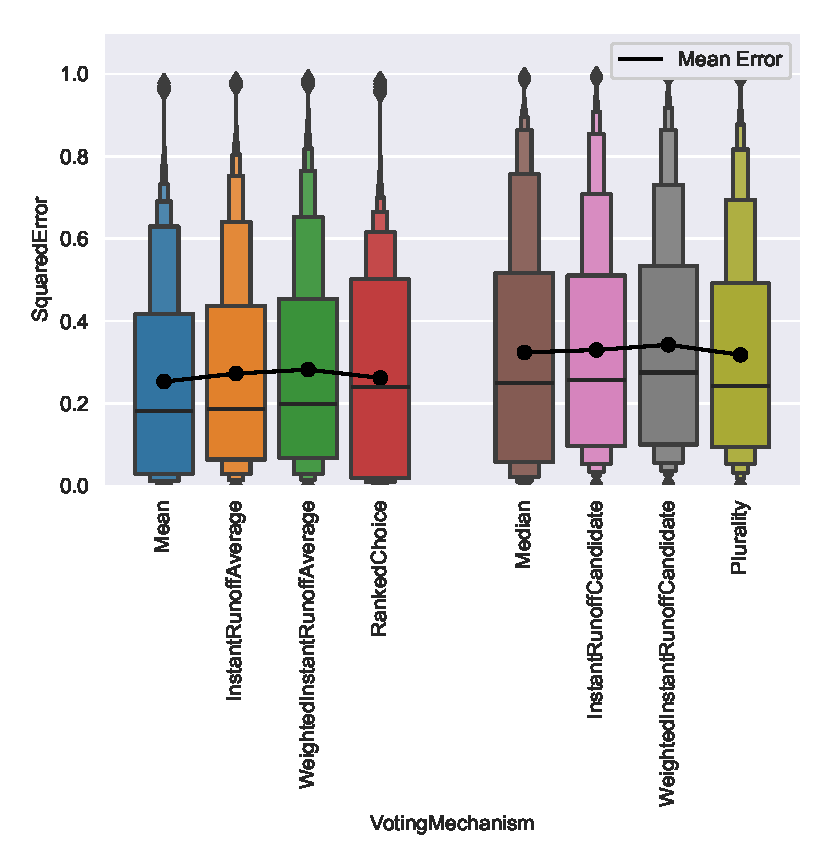
\includegraphics[scale=0.75]
    {./content/figures/voting_mechanisms/voting_mechanisms_comparison}
    \caption{Squared error populations by voting mechanism, with average
    mechanisms on the left and candidate mechanisms on the right.}
    \label{fig:voting-mechanisms-comparison}
\end{figure}

\com{It would be helpful to compare your results with what other researchers found.}

This graph immediately tells us a few things.
First, the squared error seems to be skewed, favoring numbers closer to 0.
This means there is a fairly even spread of estimates, since this is the
pattern one would expect to see from a uniform distribution of estimates.
Interestingly, however, the majority of error for most populations is
somewhere between a uniform distribution of estimates
(\autoref{fig:expected_even_distribution_squared_error}) and a normal
distribution (\autoref{fig:expected_gaussian_distribution_squared_error}).
Indeed, if the estimates are instead graphed as in
\autoref{fig:voting_mechanisms_estimate_distribution}, the distribution of estimates
is more normal than uniform.
This means most mechanisms are better at estimating \truth\ than random chance.
\com{Explain why this happens. Explain figure 3.1. I'm assuming the colors don't mean
anything?}

\begin{table}[htbp]
    % increase table row spacing, adjust to taste
    \renewcommand{\arraystretch}{1.0}

    \caption{The mean squared error for each mechanism, ordered lowest to highest.}
    \label{tab:voting-mechanism-mean-error}

    \centering
    \begin{tabular}{|c|c|}
        \hline
        Voting Mechanism                    & Mean Squared Error \\
        \hhline{|=|=|}
        Mean                                & 0.253191           \\
        \hline
        Ranked Choice                       & 0.262085           \\
        \hline
        Instant Runoff (Average)            & 0.272652           \\
        \hline
        Weighted Instant Runoff (Average)   & 0.282148           \\
        \hline
        Plurality                           & 0.318054           \\
        \hline
        Median                              & 0.323846           \\
        \hline
        Instant Runoff (Candidate)          & 0.329869           \\
        \hline
        Weighted Instant Runoff (Candidate) & 0.342495           \\
        \hline
    \end{tabular}
\end{table}

Additionally, while all distributions appear generally close, there appears to be a
slight difference between average and candidate mechanisms.
This can be confirmed by comparing the average mechanisms to the candidate mechanisms
using a U-test, with the alternative being that one population has lower error than the
other.
Performing such a test results in a p-value of 0.0, far below the $\alpha$ of 0.05.
Since candidate mechanisms can still be useful depending on the situation, both the
best average mechanisms and the best candidate mechanisms will be identified.

% \vicki{Need to define U-tests.
% It seems biased that everyone know the true value. When you know the true value, lots
% of subtle ways of cheating could get you closer. You only have a true test when the
% voters don't know the correct answer.}
Further U-tests were performed, comparing each individual voting mechanism against
every other individual mechanism.
The results of this analysis can be found in
\autoref{fig:all-voting-mechanisms-p-values}, and is further segmented and discussed in
\autoref{subsec:lowest-error-average-mechanisms} and
\autoref{subsec:lowest-error-candidate-mechanisms}.

\subsection{Average Mechanisms}\label{subsec:lowest-error-average-mechanisms}
Average mechanisms, as described in \autoref{subsubsec:average-mechanisms}, work by
averaging the estimates of the system's agents, so it is not too surprising they
result in less error than candidate mechanisms, which ultimately output only a single
agent's estimate.
However, they are not all created equally.
This leads us to the question: which average mechanisms generally work best?

To start, an ANOVA test was performed on the average mechanisms.
This produced a p-value of 0, indicating there is very likely a difference between
average mechanisms.
U-tests were then performed to compare each mechanism against every other
mechanism individually, resulting in \autoref{fig:average-mechanisms-p-values}.
The numbers next to the edges are the resultant p-values, where the alternative is
that one population has lower error than the other.
As is shown by the graph, there is sufficient evidence to reject the null hypothesis
that any of the populations are the same.

\begin{figure}[htbp]
    \centering
    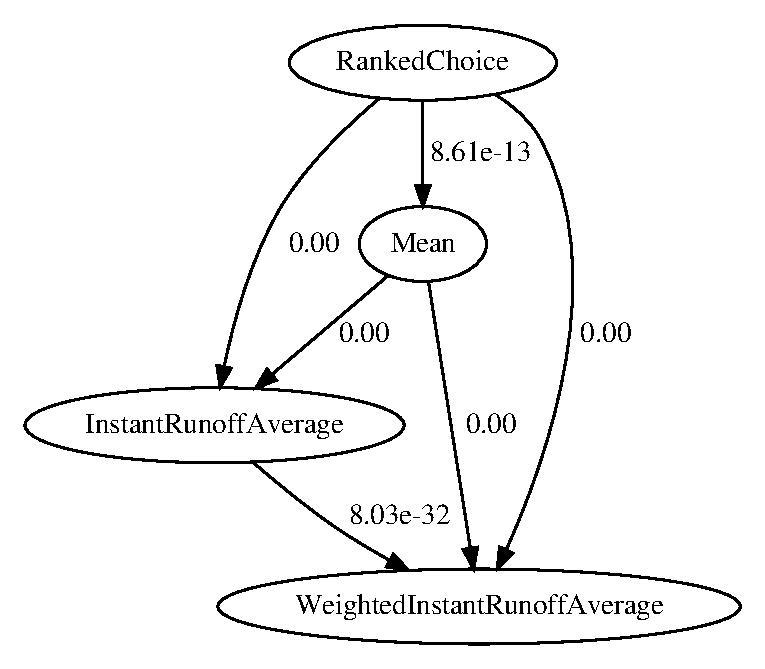
\includegraphics[scale=0.75]
    {./content/figures/voting_mechanisms/average-mechanisms-p-values.gv}
    \caption{The p-values for average voting mechanisms, given the alternative is
    that one population has lower error than the other.
    An arrow pointing to another voting mechanism indicates the `from' mechanism
    beats the `to' mechanism.}
    \label{fig:average-mechanisms-p-values}
\end{figure}

\com{Lots of zeroes in comparison. Even the non-zeroes are very near zero. Maybe I
don't know what I'm seeing. If a 0 links the types, is there a statistical difference?}

In addition, Ranked Choice appears to beat out every other voting mechanism, followed
by Mean beating two, then Weight by Instant Runoff beating one, and finally Averaged
Weighted Instant Runoff beating none.
\begin{samepage}
    This means the rankings of the average mechanisms is as follows:
    \begin{enumerate}
        \item \hyperref[para:avg-ranked-choice]{Ranked Choice}
        \item \hyperref[para:mean]{Mean}
        \item \hyperref[para:avg-instant-runoff]{Weight by Instant Runoff}
        \item \hyperref[para:avg-weighted-instant-runoff]{Averaged Weighted Instant
        Runoff}
    \end{enumerate}
\end{samepage}

\subsection{Candidate Mechanisms}\label{subsec:lowest-error-candidate-mechanisms}
Candidate voting mechanisms are described in \autoref{subsubsec:candidate-mechanisms}.
They work by selecting a single proxy as the `candidate' and using its vote as
\systemtruth.
While they do not appear to perform as well as average mechanisms, there may be
circumstances where they are required.
As such, they will still be examined to determine which candidate mechanism works best.

An ANOVA analysis was again used to start, which resulted in a p-value of
$2.49e-221$.
This, again, is clearly below $\alpha$, so the null hypothesis that all populations
are the same can be rejected.
Following the pattern of analysis in
\autoref{subsec:lowest-error-average-mechanisms}, U-tests were then performed to
identify which mechanisms produced lower error than others.
The p-values can be found in \autoref{fig:candidate-mechanisms-p-values}.

\begin{figure}[htbp]
    \centering
    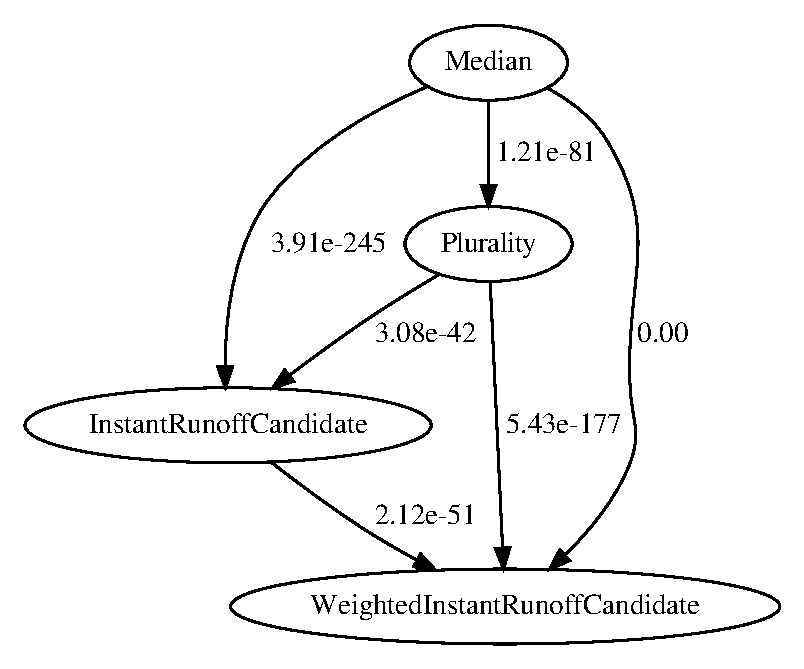
\includegraphics[scale=0.75]
    {./content/figures/voting_mechanisms/candidate-mechanisms-p-values.gv}
    \caption{The p-values for candidate voting mechanisms, given the alternative is
    that one population has lower error than the other.
    An arrow pointing to another voting mechanism indicates the `from' mechanism
    beats the `to' mechanism.}
    \label{fig:candidate-mechanisms-p-values}
\end{figure}

While not as many candidate mechanism tests yielded p-values as small as those of
the average mechanisms, there is still very strong evidence that each candidate
mechanism is different from the others.
For the candidate mechanisms, Median appears to be the best, followed
by Plurality, Instant Runoff, and finally Weighted Instant Runoff.
\begin{samepage}
    This means the rankings of the candidate mechanisms is as follows:
    \begin{enumerate}
        \item \hyperref[para:median]{Median}
        \item \hyperref[para:plurality]{Plurality}
        \item \hyperref[para:cand-instant-runoff]{Instant Runoff}
        \item \hyperref[para:cand-weighted-instant-runoff]{Weighted Instant Runoff}
    \end{enumerate}
\end{samepage}


\section{Lowest Error Weighting Mechanisms}\label{sec:lowest-error-weighting-mechanism}
Weighting mechanisms have a direct influence on how voting mechanisms operate in that
they apply weights to the estimates of the proxies.
This naturally has a direct impact on the output of a system.
\autoref{fig:weighting-mechanisms-comparison} illustrates the population of
squared error for each weighting mechanism.

\begin{figure}[htbp]
    \centering
    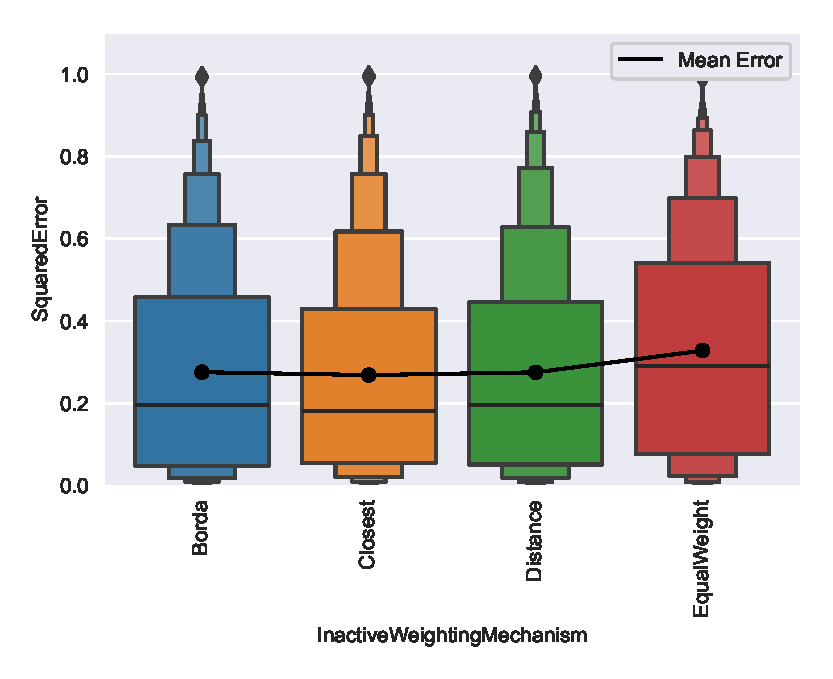
\includegraphics[scale=0.75]
    {./content/figures/weighting_mechanisms/weighting_mechanisms_comparison}
    \caption{Squared error populations by weighting mechanism.}
    \label{fig:weighting-mechanisms-comparison}
\end{figure}

\begin{table}[htbp]
    % increase table row spacing, adjust to taste
    \renewcommand{\arraystretch}{1.0}

    \caption{The mean squared error for each mechanism, ordered lowest to highest.}
    \label{tab:weighting-mechanism-mean-error}

    \centering
    \begin{tabular}{|c|c|}
        \hline
        Weighting Mechanism & Mean Squared Error \\
        \hhline{|=|=|}
        Closest             & 0.269045           \\
        \hline
        Distance            & 0.275722           \\
        \hline
        Borda               & 0.276065           \\
        \hline
        Equal Weight        & 0.328497           \\
        \hline
    \end{tabular}
\end{table}

While the mechanisms definitely appear close, there is a visible difference between
the Equal Weight mechanism and the other mechanisms.
This can be confirmed using a series of U-tests, resulting in
\autoref{fig:weighting-mechanisms-p-values}.
\begin{samepage}
    This gives us the ordering:
    \begin{enumerate}
        \item \hyperref[para:closest]{Vote for Closest}
        \item \hyperref[para:borda]{Borda}
        \item \hyperref[para:distance-voting]{Distance Voting}
        \item \hyperref[para:equal-weight]{Equal Weight}
    \end{enumerate}
\end{samepage}

\begin{figure}[htbp]
    \centering
    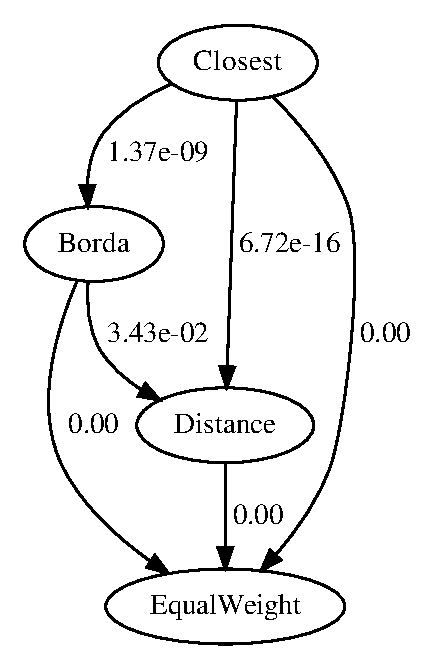
\includegraphics[scale=0.75]
    {./content/figures/weighting_mechanisms/weighting-mechanisms-p-values.gv}
    \caption{The p-values for weighting mechanisms, given the alternative is that one
    population has lower error than the other.
    An arrow pointing to another voting mechanism indicates the `from' mechanism
    beats the `to' mechanism.}
    \label{fig:weighting-mechanisms-p-values}
\end{figure}

These results are somewhat surprising in that the simplest method, arguably barring
Equal Weight, appears to produce the best results.
This may be due to the Closest mechanism yielding a lower system-wide weight while
still maintaining an ordering of preferences.
However, this does not necessarily mean the Closest mechanism pairs best with all
voting mechanisms.
This idea is explored in~\fullref{sec:lowest-error-overall-combination}.


\section{Lowest Error Combination}\label{sec:lowest-error-overall-combination}
While the previous sections have explored the lowest error for each voting mechanism and
weighting mechanism regardless of the mechanism it's paired with, this section will
explore the lowest error for each combination of voting and weighting mechanisms.

The population of error for each combination is displayed in
\autoref{fig:combined-comparison}, where a similar pattern can seen with the voting
mechanisms as what was discussed in \autoref{sec:lowest-error-voting-mechanism}: the
candidate mechanisms tend to be noticeably worse than the average mechanisms.
Additionally, average mechanisms typically produce an error below the weighting
mechanism mean, while candidate mechanisms tend to produce an error that is higher
than the mean.

\begin{figure}[htbp]
    \centering
    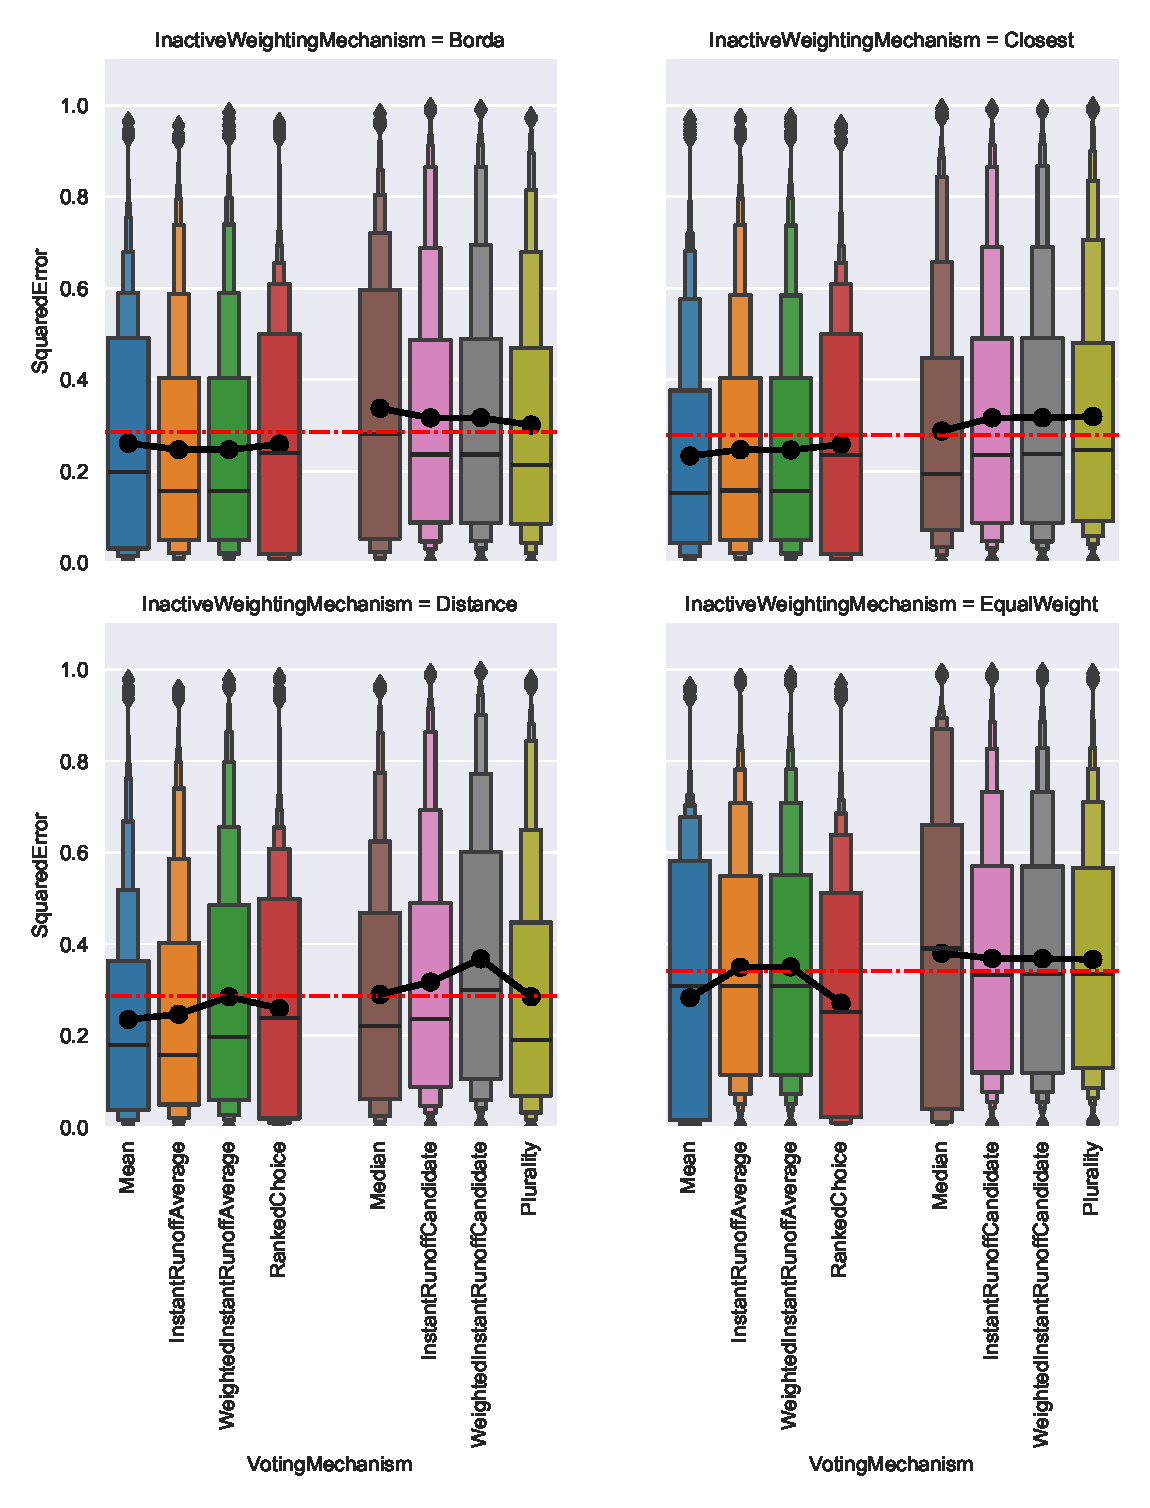
\includegraphics[scale=0.75]
    {./content/figures/combinations/combined_comparison}
    \caption{Squared error populations by combination of mechanisms. The red dashed
    line represents the mean for each weighting mechanism, while the black line with
    dots are the means for each voting mechanism using the weighting mechanism.}
    \label{fig:combined-comparison}
\end{figure}

\com{Is there a way to show all on same graph? Hard to compare between figures.}

Using U-tests, we can discover which combinations produce the lowest error.
By counting how many times any given combination beats other combinations, we can
produce an overall ranking.
The number of times one combination `beats' another by having a lower error is
displayed in \autoref{fig:combined-lesser_counts}, and is further tabulated in
\autoref{tab:combined-overall-rankings}.
From these tests, we can see the averaged easily dominate, with the first candidate
combination being in rank 15, reinforcing the idea that average mechanisms result in
lower error than candidate mechanisms.

\begin{figure}[htbp]
    \centering
    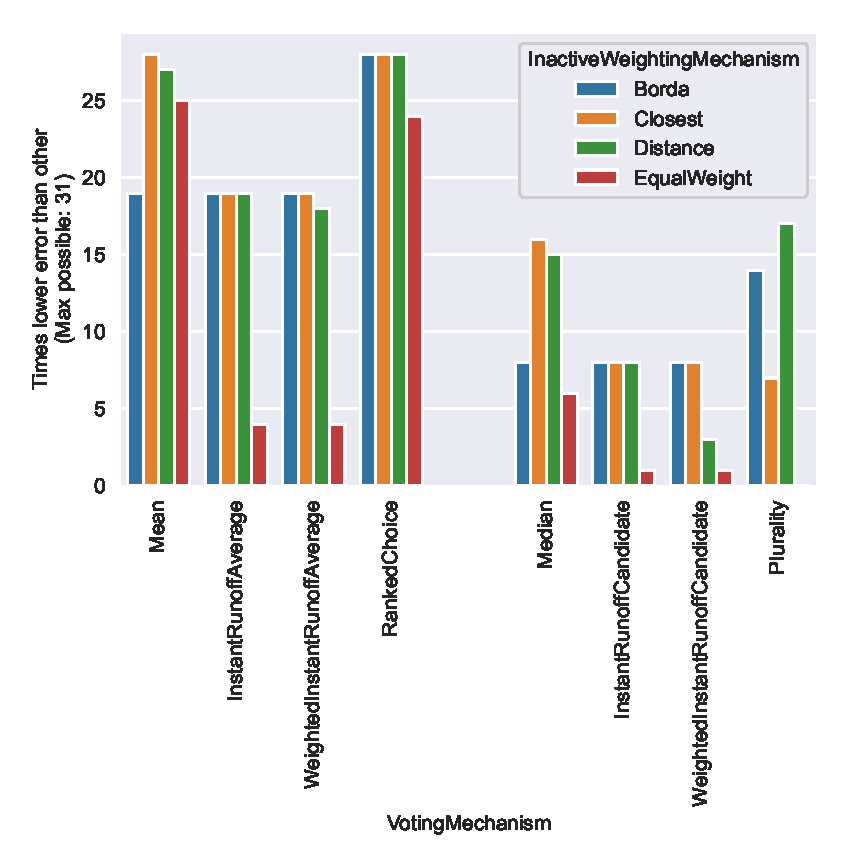
\includegraphics[scale=0.75]
    {./content/figures/combinations/combined_lesser_counts}
    \caption{The number of times each combination has a lower error according to
    U-tests.}
    \label{fig:combined-lesser_counts}
\end{figure}
\com{Why is 31 the highest? I'm not sure exactly how your test is set up. How much
lower error is significant? Number beaten seems to be a crude measure. Looking at how
others present their results would be an important sanity check. How strong is your
statistics background?}

From the graph, it can be seen that the findings
in~\fullref{sec:lowest-error-voting-mechanism} hold true with combinations of
mechanisms as well, with Ranked Choice taking the top three ranks.
The rankings from~\fullref{sec:lowest-error-weighting-mechanism} also
generally hold true, since the Closest and Borda mechanisms generally
generally hold true, since the Closest and Borda mechanisms generally
appear sooner than others.
It is possible, however, that voting mechanisms have a larger impact than weighting
mechanisms, since the general order of rankings more closely follows the voting
mechanism ordering rather than that of the weighting mechanisms.

%% I'm leaving this here in case I want to add it later. For now it seems like overkill
% Nevertheless, there may be occasions when candidate mechanisms may be preferable
% over average mechanisms, and so a deeper dive will be performed on both types of
% voting mechanisms.
%
% \subsection{Average Mechanisms}\label{subsec:lowest-error-combo-average}
%
% \subsection{Candidate Mechanisms}\label{subsec:lowest-error-combo-candidate}


\begin{table}[htbp]
    % increase table row spacing, adjust to taste
    \renewcommand{\arraystretch}{1.0}

    \caption{The rankings of combinations, ordered by the number of combinations
    beaten.
    The maximum number of combinations is 31 (32 total combinations, minus
    the combination being tested).
    Note that those with the same count are arranged in no particular order.}
    \label{tab:combined-overall-rankings}

    \centering
    \begin{tabular}{|c|c|c|}
        \hline
        Voting Mechanism                 & Weighting Mechanism & \# of Combos Beaten \\
        \hhline{|=|=|=|}
        Ranked Choice                    & Distance Voting     & 28                  \\
        \hline
        Ranked Choice                    & Closest             & 28                  \\
        \hline
        Ranked Choice                    & Borda               & 28                  \\
        \hline
        Mean                             & Closest             & 28                  \\
        \hline
        Mean                             & Distance Voting     & 27                  \\
        \hline
        Mean                             & Equal Weight        & 25                  \\
        \hline
        Ranked Choice                    & Equal Weight        & 24                  \\
        \hline
        Weight by Instant Runoff         & Borda               & 19                  \\
        \hline
        Averaged Weighted Instant Runoff & Borda               & 19                  \\
        \hline
        Weight by Instant Runoff         & Closest             & 19                  \\
        \hline
        Averaged Weighted Instant Runoff & Closest             & 19                  \\
        \hline
        Mean                             & Borda               & 19                  \\
        \hline
        Weight by Instant Runoff         & Distance Voting     & 19                  \\
        \hline
        Averaged Weighted Instant Runoff & Distance Voting     & 18                  \\
        \hline
        Plurality                        & Distance Voting     & 17                  \\
        \hline
        Median                           & Closest             & 16                  \\
        \hline
        Median                           & Distance Voting     & 15                  \\
        \hline
        Plurality                        & Borda               & 14                  \\
        \hline
        Weighted Instant Runoff          & Borda               & 8                   \\
        \hline
        Instant Runoff (Candidate)       & Distance Voting     & 8                   \\
        \hline
        Instant Runoff (Candidate)       & Closest             & 8                   \\
        \hline
        Instant Runoff (Candidate)       & Borda               & 8                   \\
        \hline
        Weighted Instant Runoff          & Closest             & 8                   \\
        \hline
        Median                           & Borda               & 8                   \\
        \hline
        Plurality                        & Closest             & 7                   \\
        \hline
        Median                           & Equal Weight        & 6                   \\
        \hline
        Averaged Weighted Instant Runoff & Equal Weight        & 4                   \\
        \hline
        Weight by Instant Runoff         & Equal Weight        & 4                   \\
        \hline
        Weighted Instant Runoff          & Distance Voting     & 3                   \\
        \hline
        Instant Runoff (Candidate)       & Equal Weight        & 1                   \\
        \hline
        Weighted Instant Runoff          & Equal Weight        & 1                   \\
        \hline
        Plurality                        & Equal Weight        & 0                   \\
        \hline
    \end{tabular}
\end{table}


\section{Weightlessly Averaging All Agents}\label{sec:weightless-average-all}
% Explain how WeightlessAverageAll works best
While the results thus far have been very interesting, this important, baseline
question remains unanswered: does employing such a system work better than simply
averaging the estimates of all agents?
Such an operation is here dubbed `weightlessly averaging all,' since it ignores
weights and simply averages all agents, including inactive agents.
Thus, this technique does not use a weighting mechanism.
\autoref{fig:weightless-voting-mechanisms-comparison} shows how weightlessly
averaging all agents compares to the other mechanisms, ignoring which weighting
mechanism is used or the distribution of the proxies or inactive agents.

\begin{figure}[htbp]
    \centering
    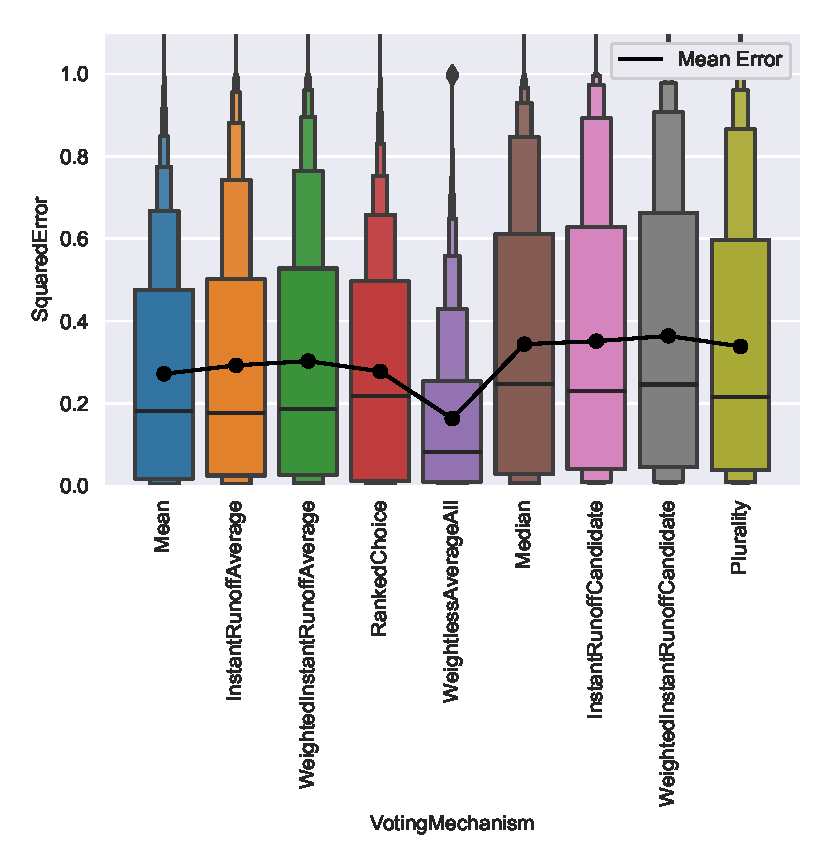
\includegraphics[scale=0.75]
    {./content/figures/weightless/weightless_voting_mechanisms_comparison}
    \caption{Squared error populations by voting mechanism, with average
    mechanisms on the left and candidate mechanisms on the right.
    Weightlessly averaging all agents' estimates is in the center.}
    \label{fig:weightless-voting-mechanisms-comparison}
\end{figure}

It is immediately evident that weightlessly averaging all agents' estimates works
considerably better that using proxy vote systems.
While this would initially indicate that proxy vote systems should not be used when a
simpler and more accurate technique already exists, this broad overview does not tell
the full story.
As explored previously, each voting mechanism is also paired with a weighting
mechanism that heavily influences its accuracy.
Additionally, we have yet to explore how the proxy and inactive estimate
distributions interact with the different mechanisms.

Indeed, performing tests on groups separated by voting and weighting mechanism, as
well as proxy and inactive estimate distribution, indicates 467 of the 2048 possible
combinations, or 22.80\%, work better using a proxy vote system than weightlessly
averaging.  \com{Why is this? If voters values are picked from a uniform
distribution, it would seem average would be accurate.}

These tests are performed as if the proxy system were used instead of weightlessly
averaging, meaning that they are performed as if the agents had the same estimate
distribution when weightlessly averaging as they did with the proxy system.

Of these 467 combinations, 223 (47.75\%) have an asymmetric proxy distribution with
a symmetric inactive distribution, while 154 (32.98\%) have an asymmetric inactive
distribution with a symmetric inactive distribution.
Additionally, 78 (16.70\%) use asymmetric distributions for both proxies and
inactive agents.
This totals to 455 (97.43\%) of the 467 more accurate proxy systems that use
asymmetric distributions!

The remaining 12 consist of high-performing voting mechanism/weighting mechanism
combinations, as discovered in \autoref{sec:lowest-error-overall-combination},
using Gaussian or \betadistribution{4}{4} distributions for the proxies,
and \betadistribution{0.3}{0.3} as the inactive distributions.  \com{Has this beta
distribution been defined in your thesis?}
These combinations are displayed in~\autoref{tab:non-asymmetric-lower-pop-systems}.

\begin{table}[htbp]
    % increase table row spacing, adjust to taste
    \renewcommand{\arraystretch}{1.0}

    \caption{The proxy voting systems that still achieve a lower error than
    weightless average all, in no particular order.}
    \label{tab:non-asymmetric-lower-pop-systems}

    \centering
    \begin{tabular}{|c|c|c|c|}
        \hline
        Voting Mechanism & %
        Weighting Mechanism & %
        Proxy Distribution & %
        Inactive Distribution \\
        \hhline{|=|=|=|=|}
        Mean & Borda & \betadistribution{4}{4} & \betadistribution{0
        .3}{0.3} \\
        \hline
        Mean & Equal Weight & \betadistribution{4}{4} & \betadistribution{0
        .3}{0.3} \\
        \hline
        Mean & Borda & Gaussian & \betadistribution{0
        .3}{0.3} \\
        \hline
        Mean & Distance & Gaussian & \betadistribution{0
        .3}{0.3} \\
        \hline
        Mean & Equal Weight & Gaussian & \betadistribution{0
        .3}{0.3} \\
        \hline
        Ranked Choice & Borda & \betadistribution{4}{4} & \betadistribution{0
        .3}{0.3} \\
        \hline
        Ranked Choice & Closest & \betadistribution{4}{4} & \betadistribution{0
        .3}{0.3} \\
        \hline
        Ranked Choice & Distance & \betadistribution{4}{4} & \betadistribution{0
        .3}{0.3} \\
        \hline
        Ranked Choice & Borda & Gaussian & \betadistribution{0
        .3}{0.3} \\
        \hline
        Ranked Choice & Closest & Gaussian & \betadistribution{0
        .3}{0.3} \\
        \hline
        Ranked Choice & Distance & Gaussian & \betadistribution{0
        .3}{0.3} \\
        \hline
        Ranked Choice & Equal Weight & Gaussian & \betadistribution{0
        .3}{0.3} \\
        \hline
    \end{tabular}
\end{table}

However, this does not mean a proxy system is always better when some distribution is
asymmetrical.
The number of lower error asymmetric combinations is only 29.62\% of the 1536
possible combinations with at least one distribution asymmetric, and all 467 lower error
combinations are only 22.80\% of all 2048 combinations.
Ten combinations with at least one asymmetric distribution failed to achieve a lower
error, regardless of the mechanism used.
These combinations are shown in \autoref{tab:no-appearance-distro-combos}.
Of note is in all these combinations, both distributions are asymmetric.
Additionally, whenever an asymmetric distribution is placed with itself, a proxy system
does not produce a lower error.
\com{What is meant by 'placed with itself'?
% TODO: Reword this sentence
% MDH: This means the proxy distribution and the inactive distribution share the same
%  asymmetric distribution
}
Finally, the more heavily skewed asymmetric distributions work worse with other
asymmetric distributions.

\begin{table}[htbp]
    % increase table row spacing, adjust to taste
    \renewcommand{\arraystretch}{1.0}

    \caption{The asymmetric distribution combinations that were never found to achieve
    lower error than weightlessly averaging, arranged in no particular order.}
    \label{tab:no-appearance-distro-combos}

    \centering
    \begin{tabular}{|c|c|}
        \hline
        Proxy Distribution        & Inactive Distribution     \\
        \hhline{|=|=|}
        \betadistribution{0.3}{3} & \betadistribution{0.3}{3} \\
        \hline
        \betadistribution{0.3}{3} & \betadistribution{3}{0.3} \\
        \hline
        \betadistribution{0.3}{3} & \betadistribution{4}{1}   \\
        \hline
        \betadistribution{1}{4}   & \betadistribution{1}{4}   \\
        \hline
        \betadistribution{1}{4}   & \betadistribution{4}{1}   \\
        \hline
        \betadistribution{3}{0.3} & \betadistribution{0.3}{3} \\
        \hline
        \betadistribution{3}{0.3} & \betadistribution{1}{4}   \\
        \hline
        \betadistribution{3}{0.3} & \betadistribution{3}{0.3} \\
        \hline
        \betadistribution{4}{1}   & \betadistribution{1}{4}   \\
        \hline
        \betadistribution{4}{1}   & \betadistribution{4}{1}   \\
        \hline
    \end{tabular}
\end{table}

The natural next question that aries is, `which mechanism combinations are more likely
to produce a lower error?'
The count of how many times each voting/weighting mechanism combination
tests to have a lower error than weightlessly averaging is tabulated
in~\autoref{tab:lower-pop-combo-count}.
This table would seem to indicate that the stronger combinations, as explored
in~\fullref{sec:lowest-error-overall-combination}, are more able to achieve a lower
error.
Surprisingly, even candidate mechanisms are occasionally able to achieve a lower error
as well.

\begin{table}[htbp]
    % increase table row spacing, adjust to taste
    \renewcommand{\arraystretch}{1.0}

    \caption{The count of mechanism combinations that achieve a lower error
    population than weightlessly averaging, ordered first by count, then by voting
    mechanism, and finally by weighting mechanism.}
    \label{tab:lower-pop-combo-count}

    \centering
    \begin{tabular}{|c|c|c|}
        \hline
        Voting Mechanism                    & Weighting Mechanism & Count \\
        \hhline{|=|=|=|}
        Mean                                & Equal Weight        & 20    \\
        \hline
        Plurality                           & Closest             & 20    \\
        \hline
        Ranked Choice                       & Borda               & 20    \\
        \hline
        Ranked Choice                       & Closest             & 20    \\
        \hline
        Ranked Choice                       & Distance            & 20    \\
        \hline
        Ranked Choice                       & Equal Weight        & 19    \\
        \hline
        Instant Runoff (Average)            & Borda               & 16    \\
        \hline
        Instant Runoff (Average)            & Closest             & 16    \\
        \hline
        Instant Runoff (Average)            & Distance            & 16    \\
        \hline
        Mean                                & Borda               & 16    \\
        \hline
        Mean                                & Closest             & 16    \\
        \hline
        Median                              & Closest             & 16    \\
        \hline
        Weighted Instant Runoff (Average)   & Borda               & 16    \\
        \hline
        Weighted Instant Runoff (Average)   & Closest             & 16    \\
        \hline
        Instant Runoff (Average)            & Equal Weight        & 14    \\
        \hline
        Instant Runoff (Candidate)          & Borda               & 14    \\
        \hline
        Instant Runoff (Candidate)          & Closest             & 14    \\
        \hline
        Instant Runoff (Candidate)          & Distance            & 14    \\
        \hline
        Median                              & Equal Weight        & 14    \\
        \hline
        Plurality                           & Distance            & 14    \\
        \hline
        Weighted Instant Runoff (Average)   & Equal Weight        & 14    \\
        \hline
        Weighted Instant Runoff (Candidate) & Borda               & 14    \\
        \hline
        Weighted Instant Runoff (Candidate) & Closest             & 14    \\
        \hline
        Instant Runoff (Candidate)          & Equal Weight        & 13    \\
        \hline
        Weighted Instant Runoff (Candidate) & Equal Weight        & 13    \\
        \hline
        Mean                                & Distance            & 11    \\
        \hline
        Plurality                           & Equal Weight        & 11    \\
        \hline
        Median                              & Borda               & 10    \\
        \hline
        Weighted Instant Runoff (Average)   & Distance            & 10    \\
        \hline
        Weighted Instant Runoff (Candidate) & Distance            & 10    \\
        \hline
        Median                              & Distance            & 8     \\
        \hline
        Plurality                           & Borda               & 8     \\
        \hline
    \end{tabular}
\end{table}

While it is clear that simply weightlessly averaging all agent's estimates is a more
accurate method, there appear to be occasions when proxy vote systems can reduce
error, particularly when one of the error distributions is asymmetrical.
\com{This doesn't appear to match your previous discussion where you list all the
ones better than weightlessly averaging.}
This view into distributions and other parameters begs for a closer look and may yield
fascinating results upon closer inspection.


\section{How many Agents to Use}\label{sec:how-many-agents}
Regardless of which combination of mechanisms is used, the question still remains,
`How many proxies and inactive agents should be used?'
This question directly affects the cost of a system, since the cost is tied to the
number of agents, and so ideally the number of agents should be minimized.

There are three parts to this question, all of which will be addressed here.
The first is how many proxies should be used.
\autoref{fig:proxy-count} shows how proxy count affects the error of a system.
From this graph, we can see in the beginning more proxies produces better results.
However, this benefit reduces over time \com{It isn't really over time is it? It
seems the value decreases with increased proxies. If you are weightlessly averaging
all, why doesn't that get worse with more proxies? Doesn't weightlessly averaging
all, mean all voters or just all proxies? Must mean the latter.
% TODO: Rephrase this
% MDH: Whoops, definitely should not be over time. I meant as the x axis increases,
% meaning with increased proxies. Specifically, the benefit of adding another proxy
% shrinks as more proxies are added. E.g. adding 1 more proxy when I have 100 does not
% give as much benefit as adding 1 when I have 10.
} and eventually
flattens out or, in the case
of some combinations, increases the error of a system.
This benefit seems to bottom out between 10 and 15 proxies.

\begin{figure}[htbp]
    \centering
    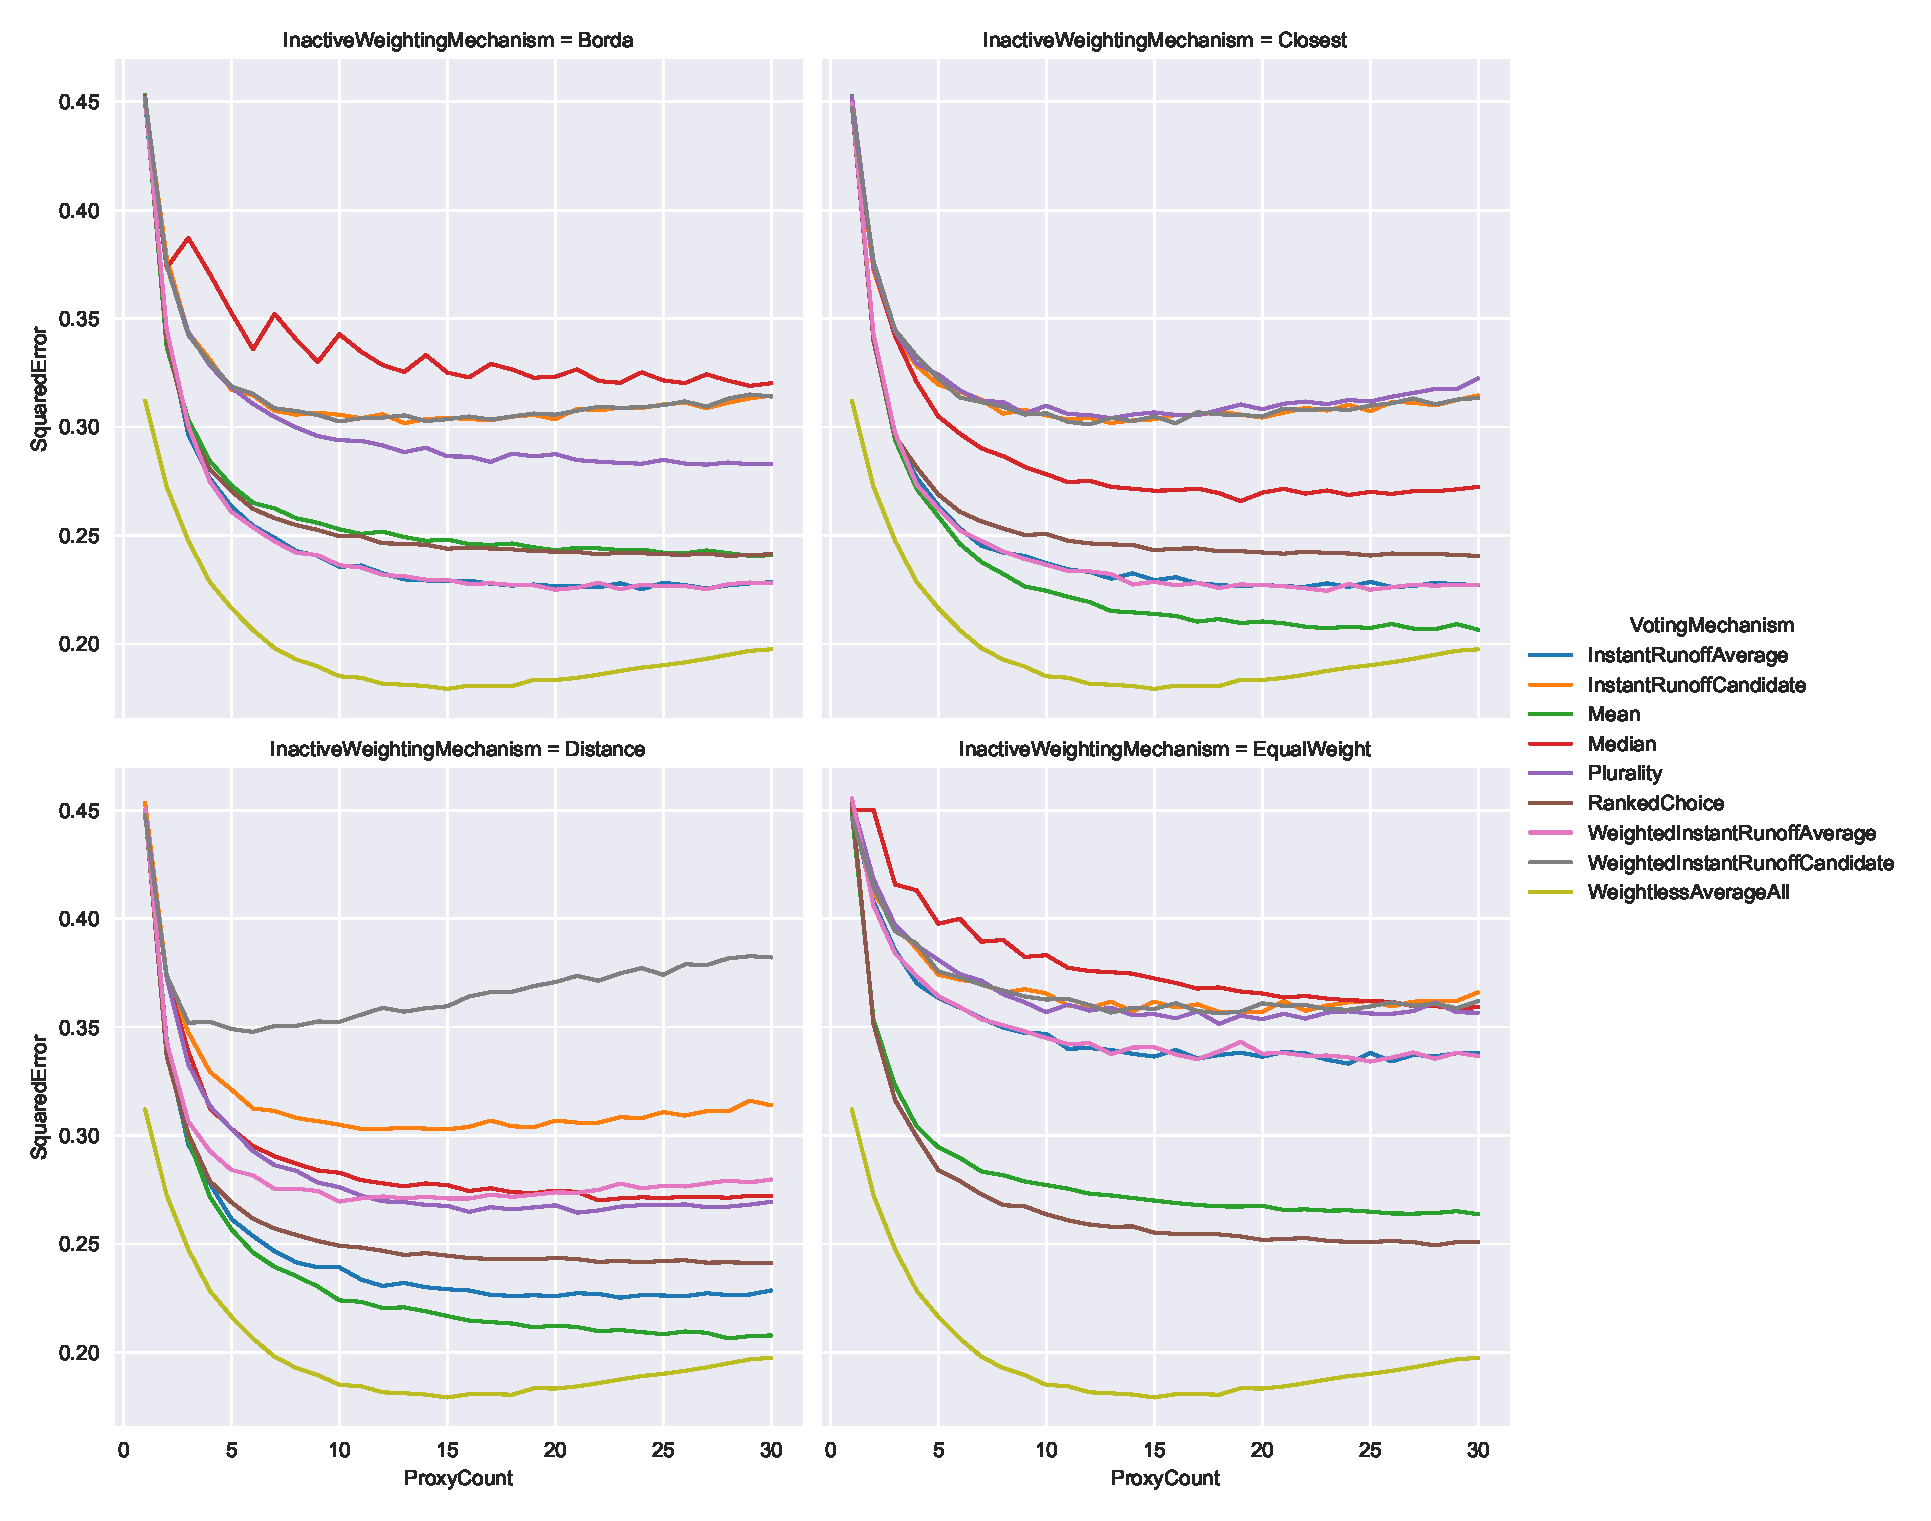
\includegraphics[
        width=\textwidth,
        height=\dimexpr
        \textheight - 4 % Could also be .9\textheight
        \baselineskip,
        keepaspectratio]
    {./content/figures/ratios/proxy_count}
    \caption{How the number of proxies affects the system error.}
    \label{fig:proxy-count}
\end{figure}
\com{Hard to read all the different colors. Maybe also use dotted/dashed line types.}

The second part of determining how many agents to use is how many inactive agents to
use.
As with minimizing the number of proxies, minimizing the number of inactive agents to
use will help reduce the costs of the system.
\autoref{fig:inactive-count} seems to indicate that, with the exception of
weightlessly averaging all agents, there is little benefit in using more inactive
agents.
This doesn't mean only one inactive agent should be used, as is indicated by the
third part of the question: the ratio between proxies and inactive agents.

\begin{figure}[htbp]
    \centering
    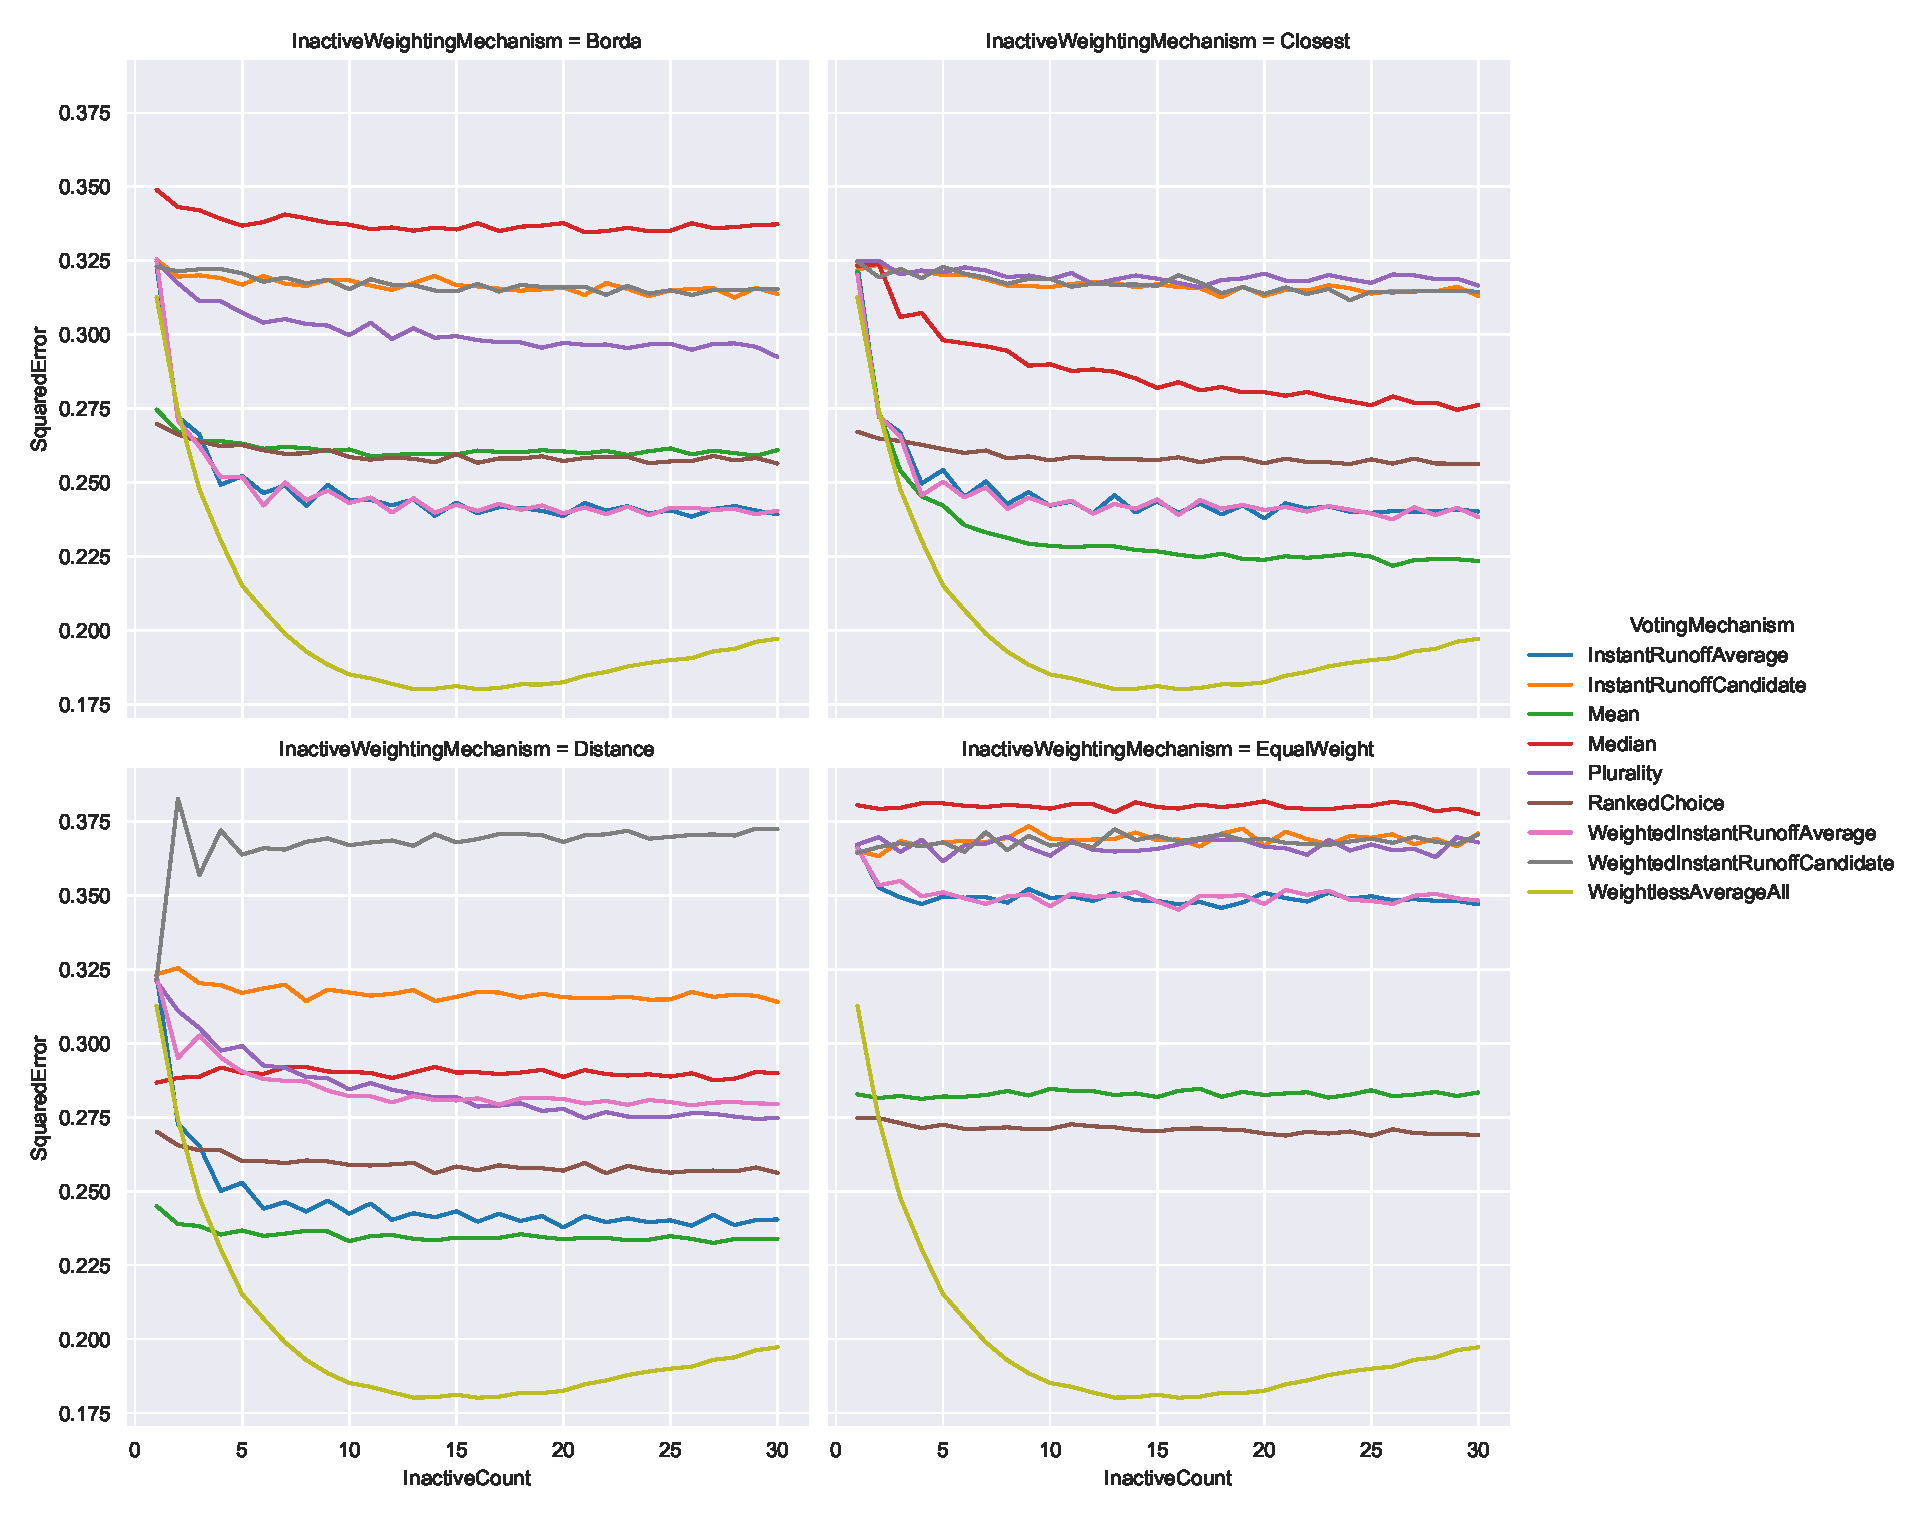
\includegraphics[
        width=\textwidth,
        height=\dimexpr
        \textheight - 4 % Could also be .9\textheight
        \baselineskip,
        keepaspectratio]
    {./content/figures/ratios/inactive_count}
    \caption{How the number of inactive agents affects the system error.}
    \label{fig:inactive-count}
\end{figure}

\autoref{fig:ratios}~and~\ref{fig:ratios-zoomed} display the error in the system as
the ratio between proxies and inactive agents increases, with
\autoref{fig:ratios-zoomed} providing a zoomed-in perspective.
Interestingly, the curve produced in each of these graphs flattens around a 1:1
ratio, indicating that there is little or no benefit to having a differing number of
proxies and inactive agents.
Additionally, there seems to be small `hiccups' at each whole number.  \com{I don't
think this can be glossed over.  }
While the reason behind the hiccups is not explored here, this would indicate that a
slightly higher or lower ratio than 1:1 should be used.
With this mind, and since the number of inactive agents generally does not have an
effect on the system error, it would likely be best to use slightly fewer inactive
agents than proxies in an effort to decrease the total system cost while still
maintaining accuracy.

\begin{figure}[htbp]
    \centering
    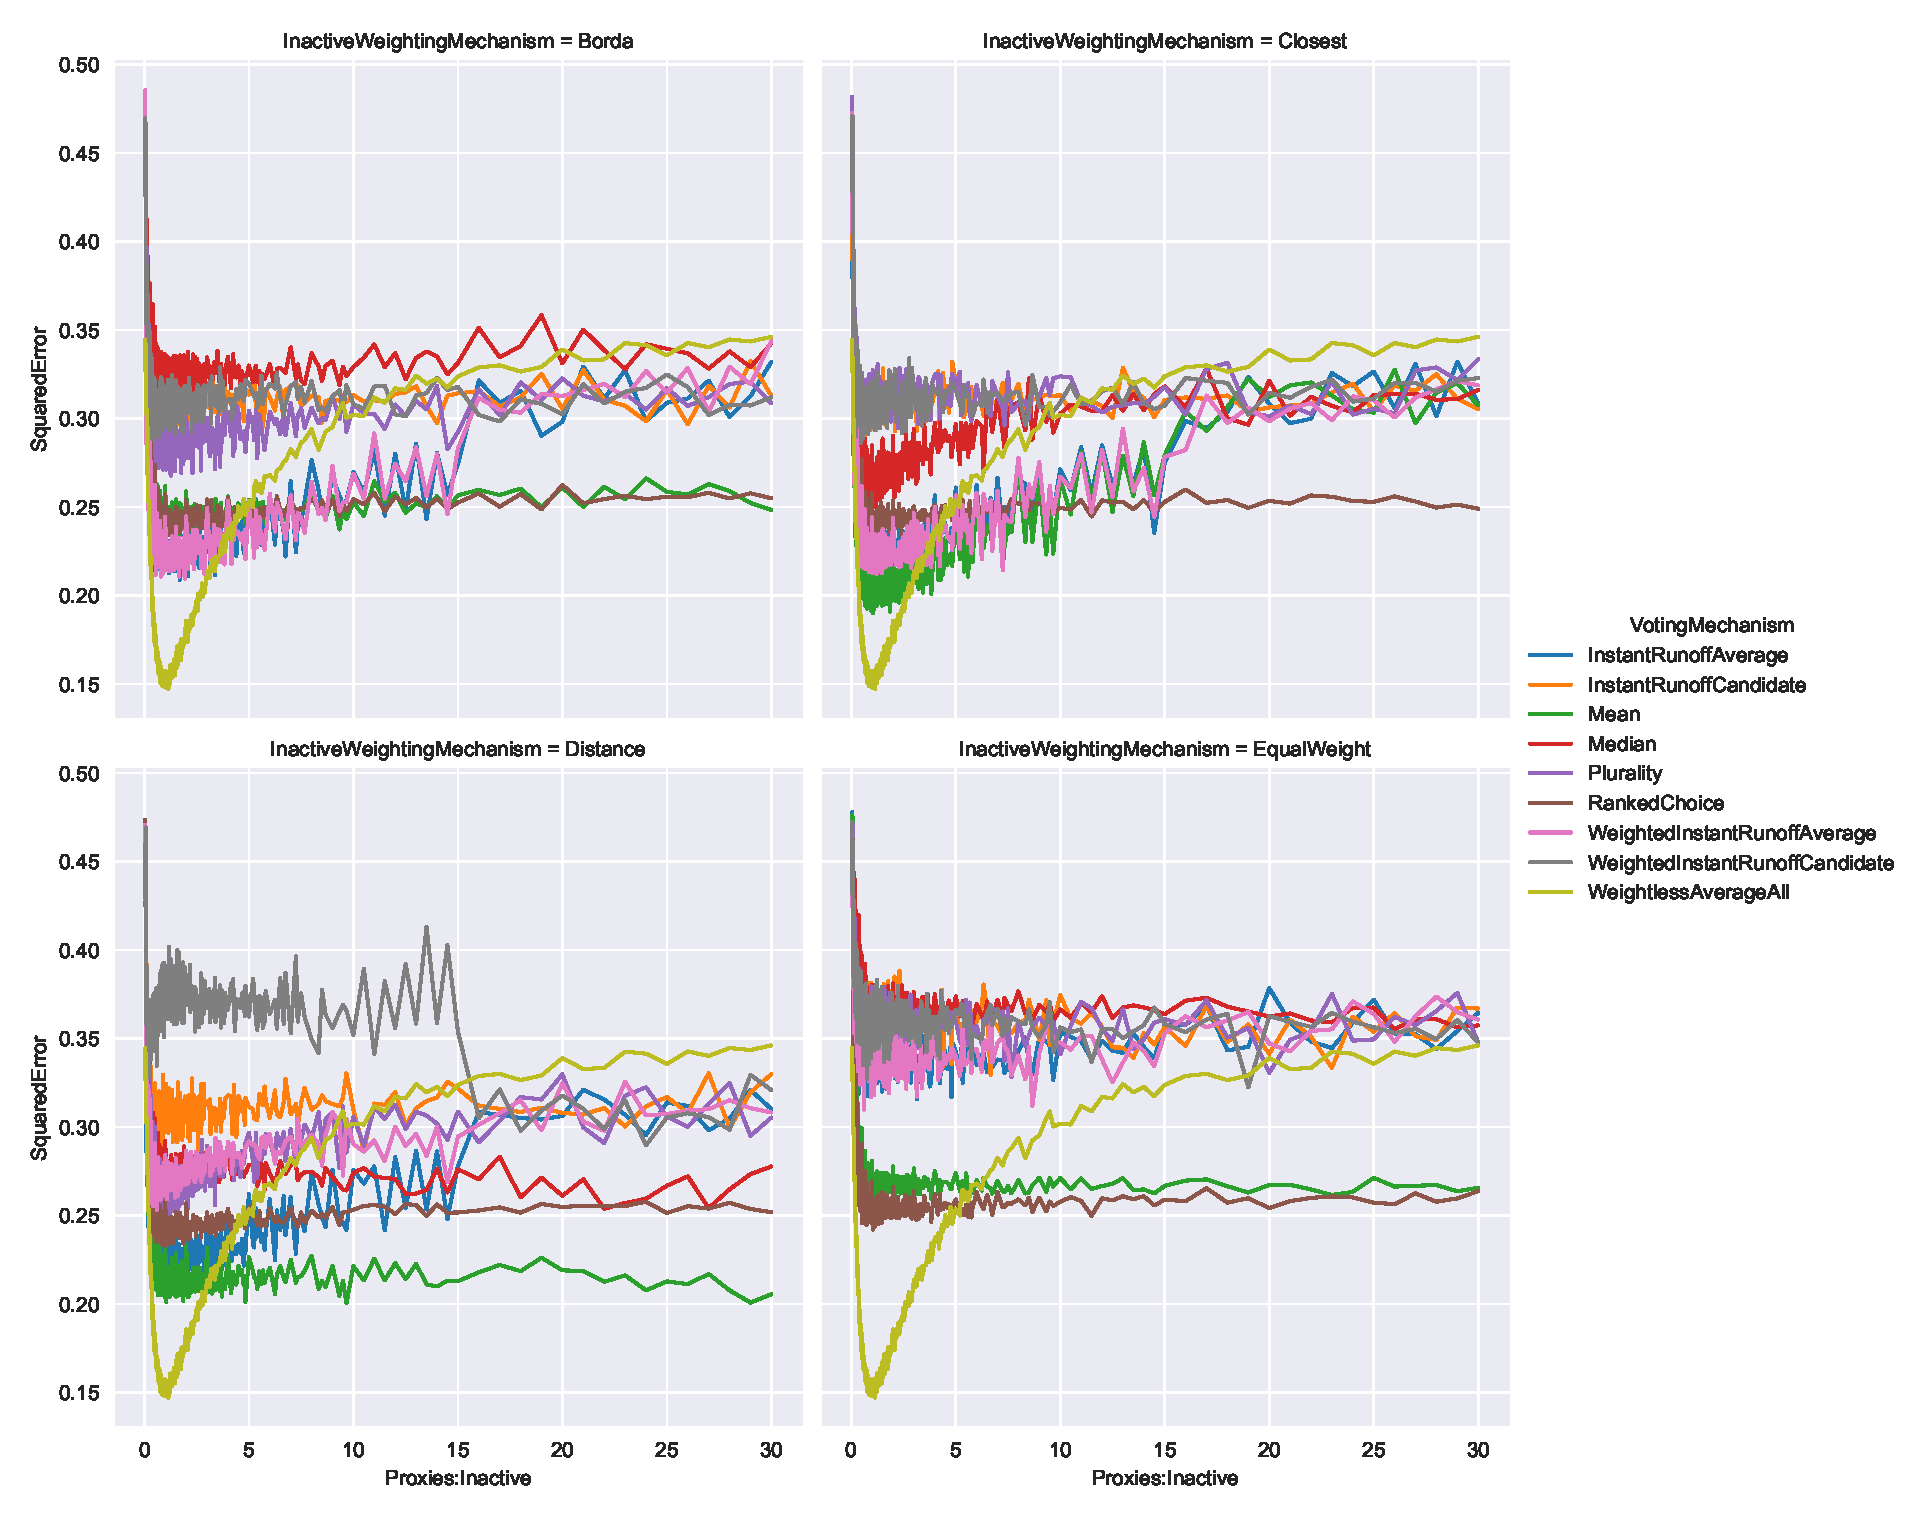
\includegraphics[
        width=\textwidth,
        height=\dimexpr
        \textheight - 4 % Could also be .9\textheight
        \baselineskip,
        keepaspectratio]
    {./content/figures/ratios/ratios}
    \caption{How the ratio between proxies and inactive agents affects the system
    error.}
    \label{fig:ratios}
\end{figure}
\com{I don't understand why the weighlessaverageAll is so erratic and poor.
% Weighless average all is poor in terms of error, meaning it has low error. The closer
% to zero, the better.
% It's probably erratic because I didn't smooth the curve.
}

\begin{figure}[htbp]
    \centering
    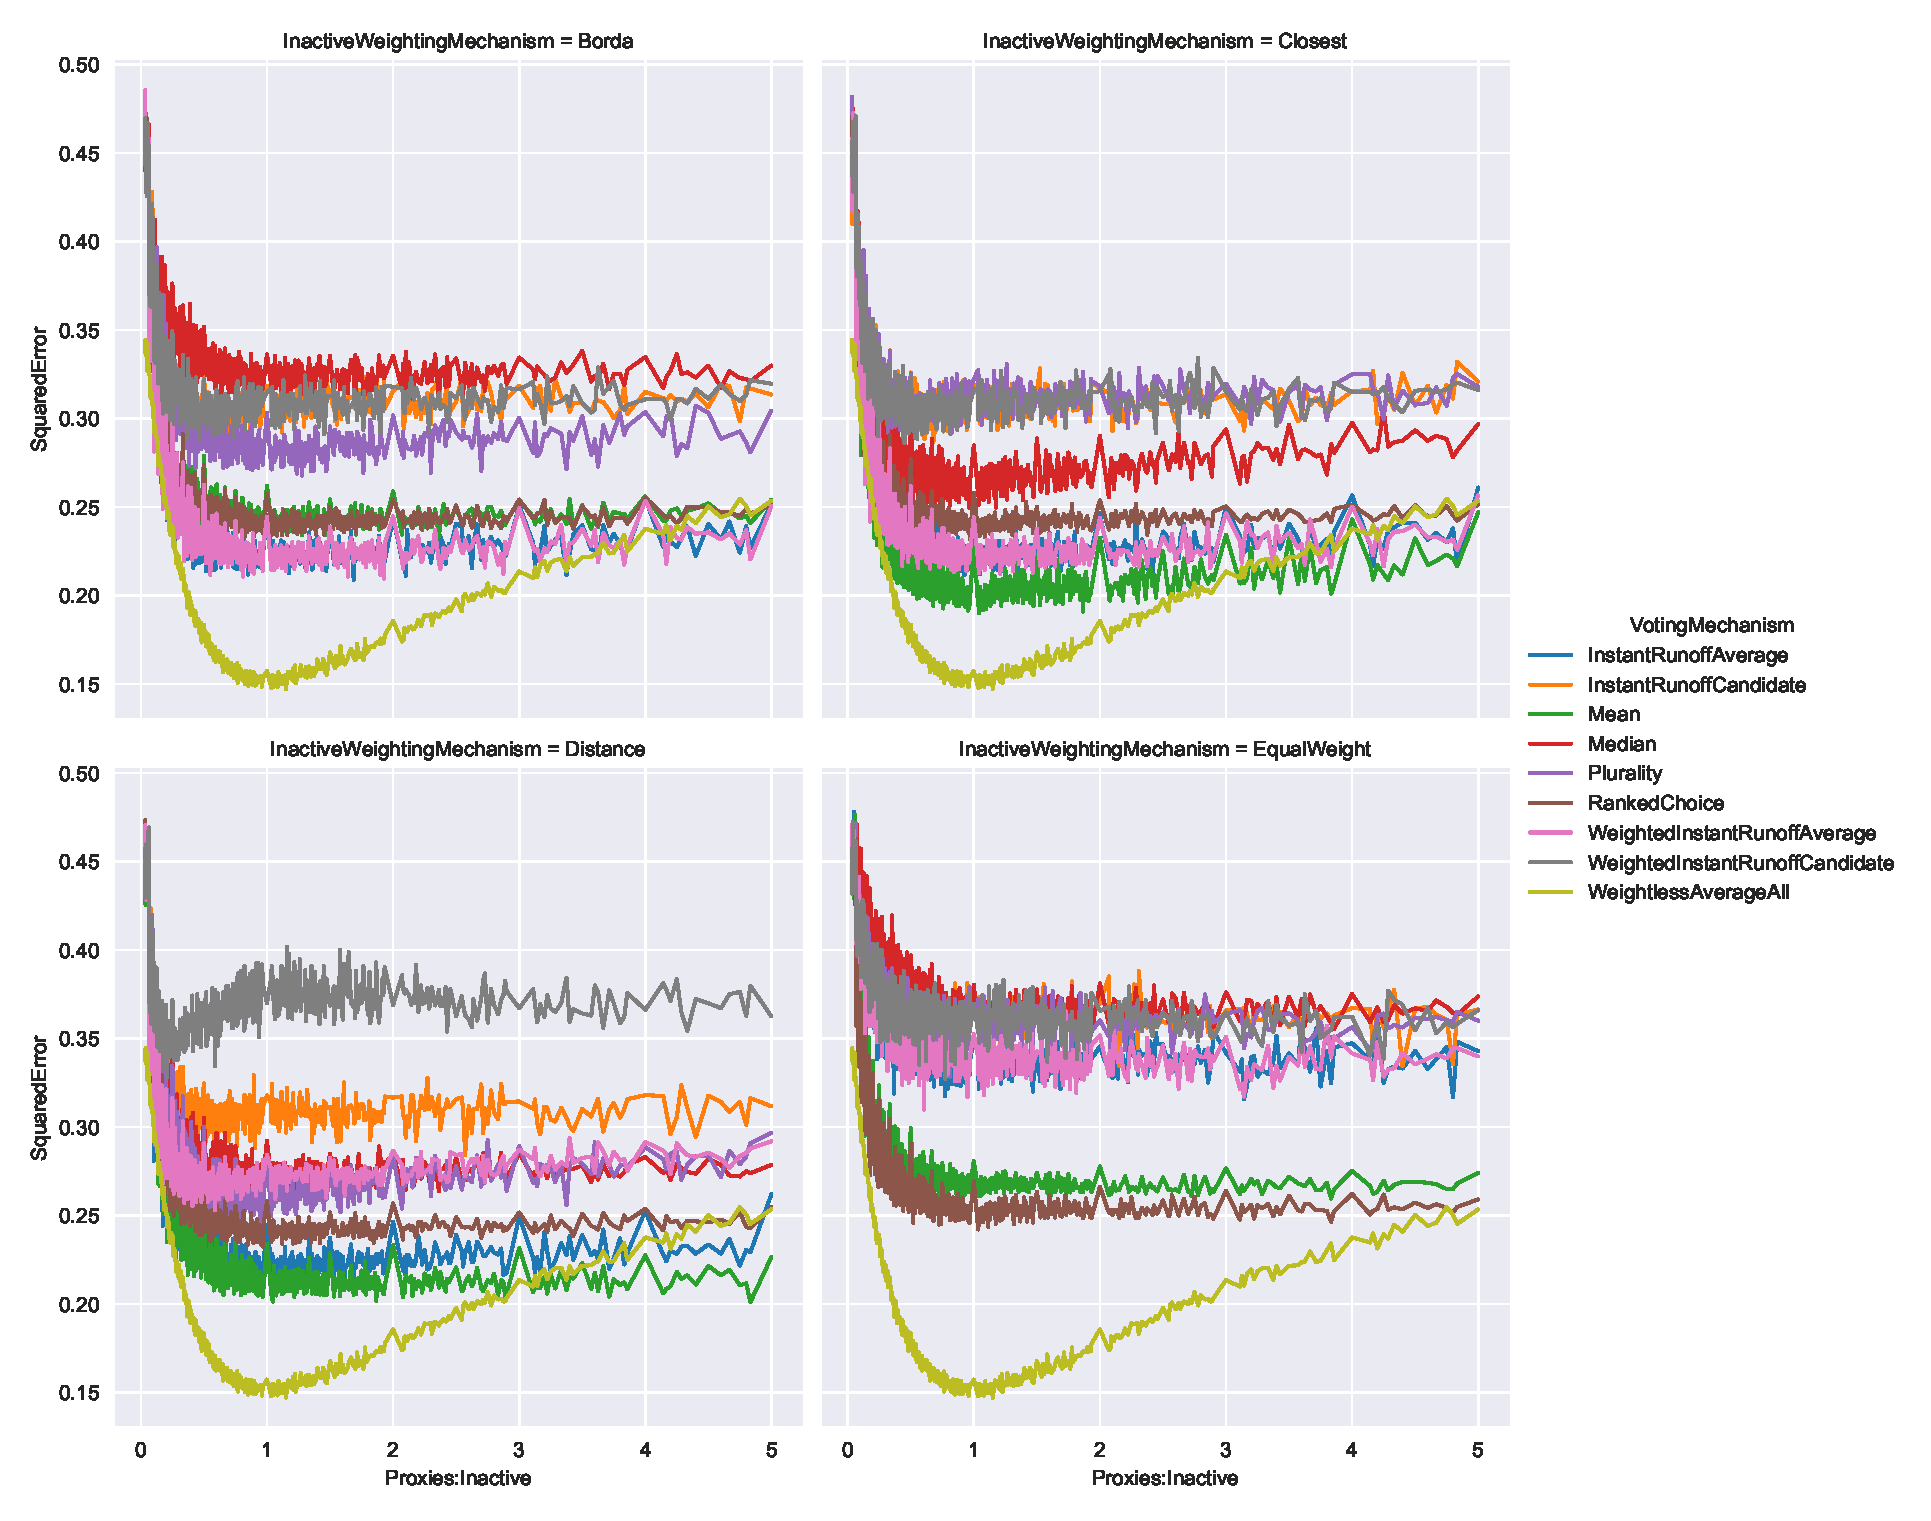
\includegraphics[
        width=\textwidth,
        height=\dimexpr
        \textheight - 4 % Could also be .9\textheight
        \baselineskip,
        keepaspectratio]
    {./content/figures/ratios/ratios_zoomed}
    \caption{How the ratio between proxies and inactive agents affects the system
    error. Zoomed in to better see the curve.}
    \label{fig:ratios-zoomed}
\end{figure}

    % %
%  This document contains chapter 4 of the thesis.
%

\chapter{CONCLUSIONS AND FURTHER WORK}\label{ch:conclusions-and-further-work}

\section{Conclusions}\label{sec:conclusions}
Proxy vote systems as a method to increase system accuracy are situational tools.
This technique is best used when one of the distributions of error is asymmetrical,
and thus require the expected distribution of error to be known.
However, under the correct circumstances a proxy vote system can be used to increase
the accuracy of a system.
Additionally, not all proxy vote systems are created equally and some combinations of
voting and weighting mechanisms can be more effective than others.
As such, the proxy vote system and the mechanisms used should be chosen after
understanding the problem for which the system is desired to solve.

Furthermore, the ratio between proxies and inactive agents should be chosen well.
As previously shown, all systems, including weightlessly averaging all agents, benefit
from an appropriate number of agents.
As discussed in~\fullref{sec:how-many-agents}, this sweet spot appears to be between
10 and 15 proxies, with slightly more or less inactive agents.
This may cause using such techniques to be too expensive if it is not possible to use
sufficiently cheap proxies and inactive agents.
However, if such agents are available the proxy vote or weightless average approach
may be able to achieve better performance than alternative techniques that cost more
than the combined sum of the agents used.

Overall, proxy vote systems as a method to increase system accuracy appears to show
promise under some circumstances.
Further research may be required to identify its full capabilities and weaknesses
before its full potential can be exploited.

\section{Further Work and Improvements}\label{sec:further-work-and-improvements}
% FIXME: This might need to be moved to Chapter 4
% - Multiple levels of expertise. Expert voters could have varying levels of
% accuracy, allowing for more complex systems.
% - (If I decide to restrict experts and untrained to the same mins and maxes)
% Allow for untrained to have a lower restriction, making them less accurate.
% - Independently track time, monetary cost, etc. for system cost (described
% in the cost section of Criteria. Useful identifying multiple systems for
% different costs.
% Closer look into instances where proxy voting works better than weightlessly averaging


    % Endmatter
    % For BibTeX references: specify a .bib file and a style.
    % The style used here is for IEEE transactions formatting:
    \references{
        references/IEEEabrv,
        references/research}
    {IEEEtran}

    % The style used here is for AIAA formatting:
%    \references{IEEEabrv,sample}{aiaa}

    % %
%  Example Appendix pages.
%  Modified to use new usu-thesis-mk2 appendix facilities.
%
%  Time-stamp: "[appendix.tex] last modified by Scott Budge (scott) on
%  2021-06-28 (Monday, 28 June 2021) at 09:03:44 on goga.ece.usu.edu"
%
%  Info: $Id: appendix.tex 1183 2021-06-28 16:49:30Z scott $   USU
%  Revision: $Rev: 1183 $
% $LastChangedDate: 2021-06-28 10:49:30 -0600 (Mon, 28 Jun 2021) $
% $LastChangedBy: scott $
%
%
% For a single appendix, use \makeappendix, and place the 
% body of the appendix after it

%\makeappendix

% < single appendix body here >

% For multiple appendices, use \makeappendices, and create each appendix
% using \appendix{}
% For sub-appendices use \appendixsection{} and \appendixsubsection{}

\makeappendices
\appendix{Voting Distributions}\label{chap:voting-distributions}

\appendixsection{Percent inside Extents}
% TODO: Add description of table
This is placeholder text to ensure
\autoref{tab:distributions-percent-inside-extents} stays in the correct
location. % FIXME

% - Distribution of votes
%     - Uniform
%     - Gaussian
%     - Bimodal about center
%     - Skewed?

\begin{table}[htbp]
    % increase table row spacing, adjust to taste
    \renewcommand{\arraystretch}{1.3}

    \caption{List of distributions used by agents to vote.}
    \label{tab:distributions-percent-inside-extents}

    \centering
    \begin{tabular}{|c|c|c|}
        \hline
        Distribution      & Notation      & Percent inside Extents \\
        \hline
        Uniform           & \uniformdist  & 100\%                  \\
        \hline
        Normal (Gaussian) & \gaussiandist & 99.7\%                 \\
        \hline
        Beta              & \betadist     & 100\%                  \\
        \hline
    \end{tabular}
\end{table}

\appendixsection{Distributions used}
% TODO: Add graphs of distributions used
\begin{table}[htbp]
    % increase table row spacing, adjust to taste
    \renewcommand{\arraystretch}{1.3}

    \caption{List of distributions used by agents to vote.}
    \label{tab:distributions}

    \centering
    \begin{tabular}{|c|c|c|}
    \end{tabular}
\end{table}

\appendixsection{Voting Mechanism P-Values}
\autoref{fig:all-voting-mechanisms-p-values} illustrates the p-values for all voting
mechanisms, given the alternative is one population is lesser than the other.
An arrow pointing to another voting mechanism indicates the `from' mechanism beats
the `to' mechanism.

\begin{figure}[!t]
    \centering
    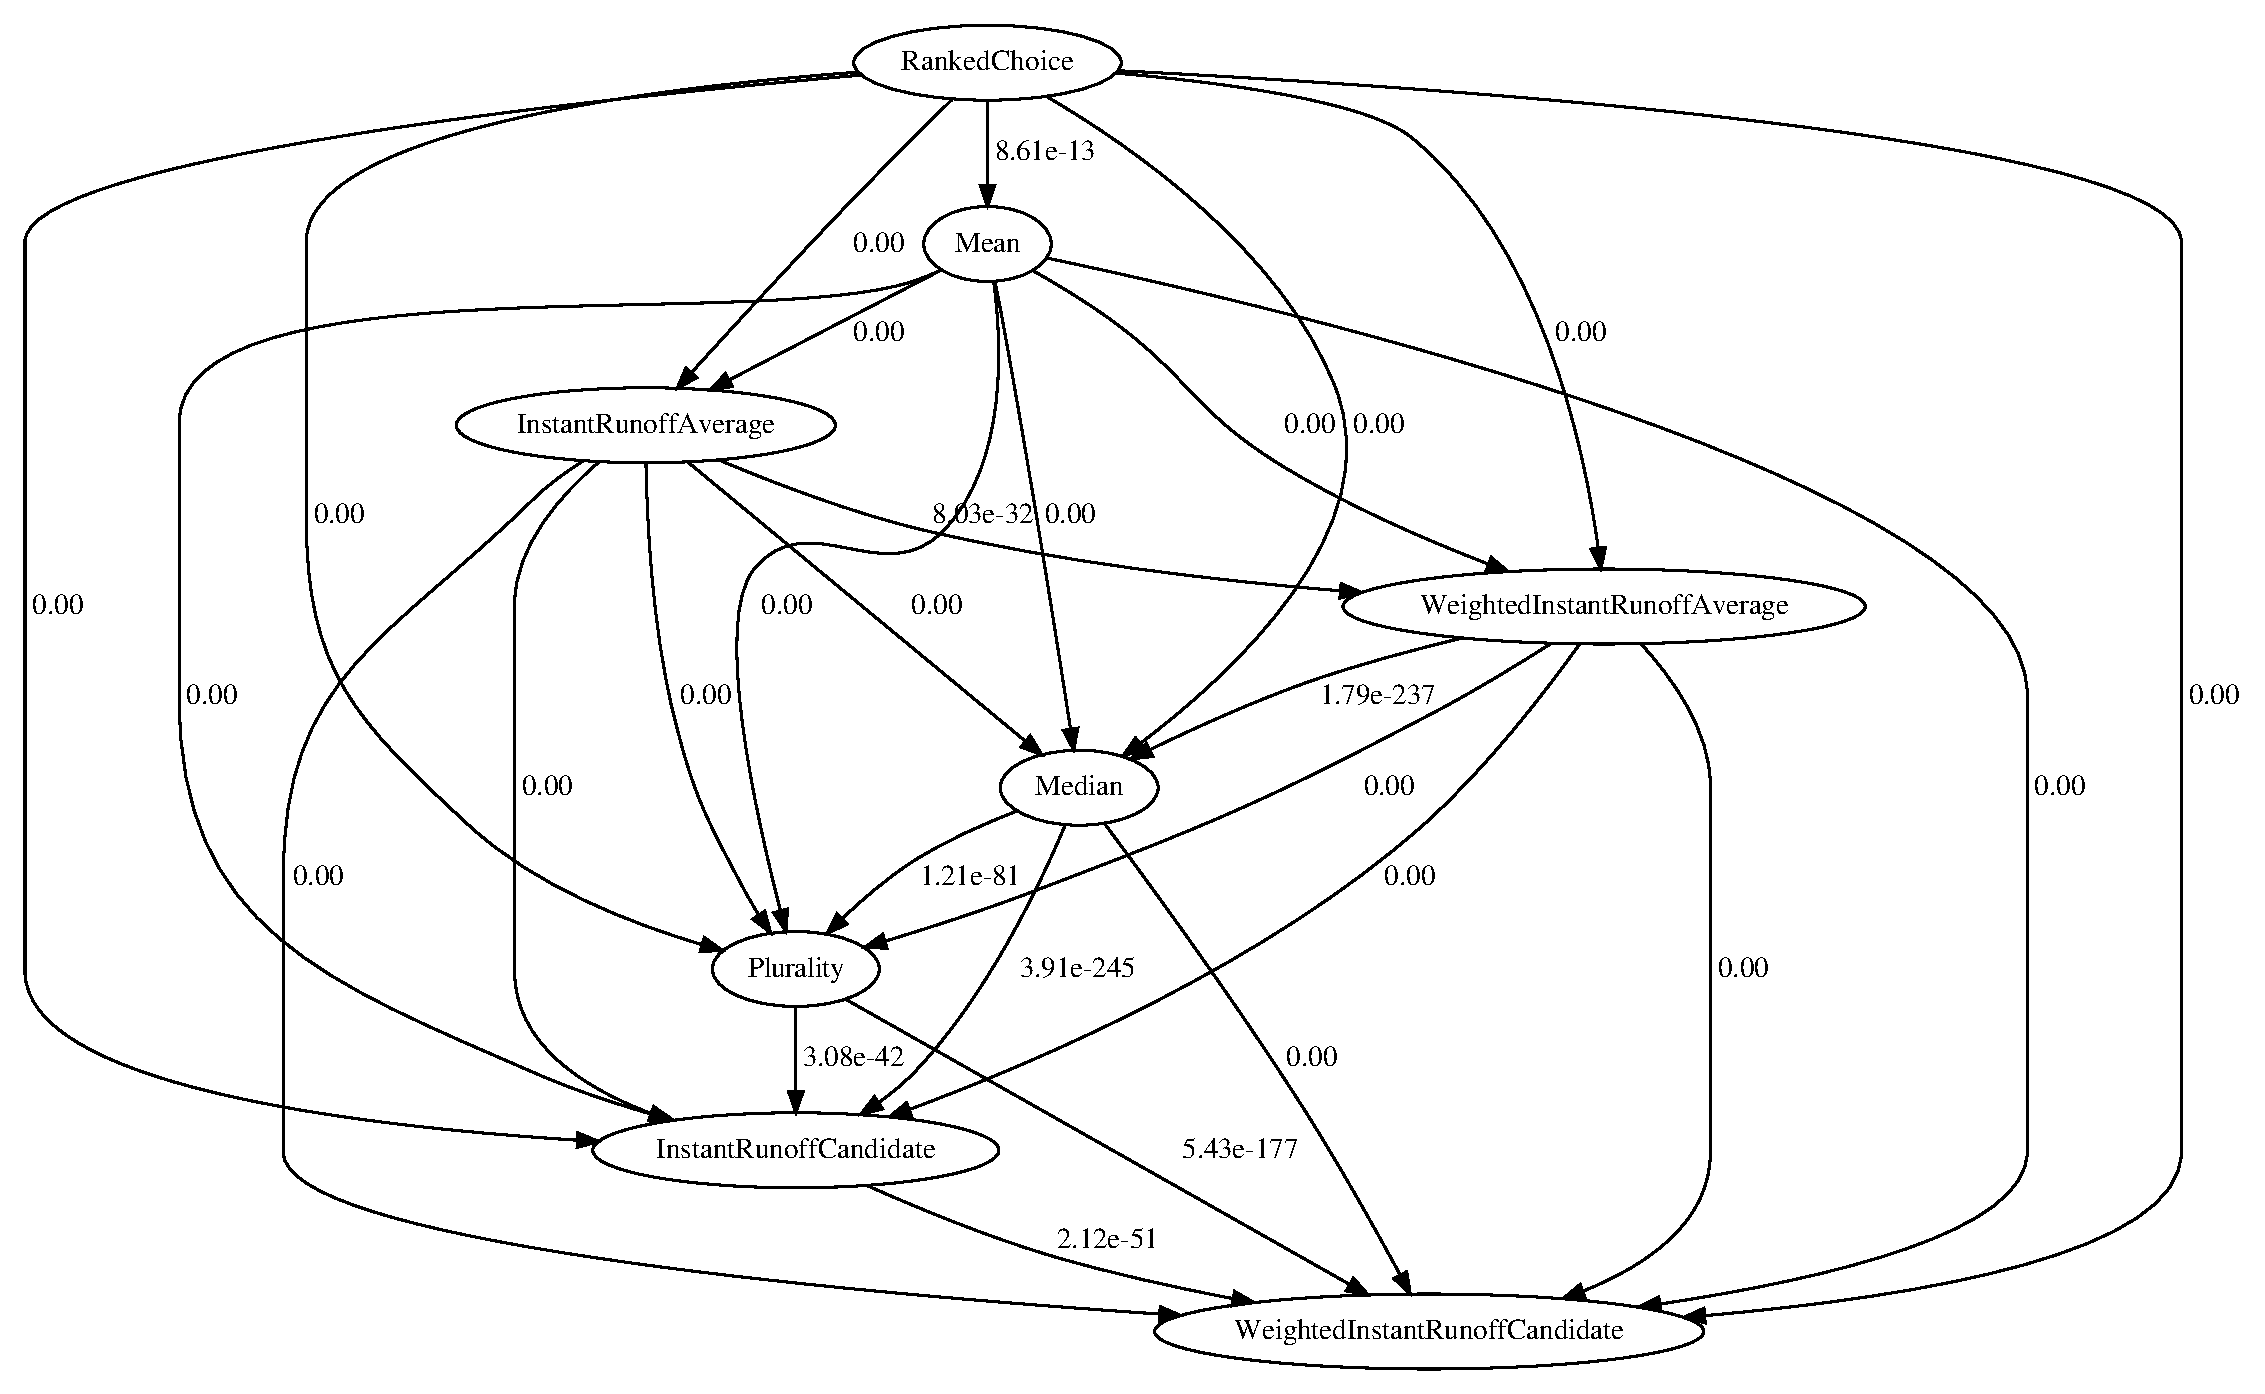
\includegraphics[
        angle=90,
        width=\textwidth,
        height=\dimexpr
        \textheight - 4 % Could also be .9\textheight
        \baselineskip,
        keepaspectratio]
    {./content/figures/voting_mechanisms/all-voting-mechanisms-p-values.gv}
    \caption{The p-values for all voting mechanisms, given the alternative is one
    population is lesser than the other.
    An arrow pointing to another voting mechanism indicates the `from' mechanism beats
    the `to' mechanism.}
    \label{fig:all-voting-mechanisms-p-values}
\end{figure}


\appendixsection{Distributions of Variables}
The distribution of variables for each voting mechanism is displayed as a
KDE graph in the figures of this section.

\begin{figure}[!t]
    \centering
    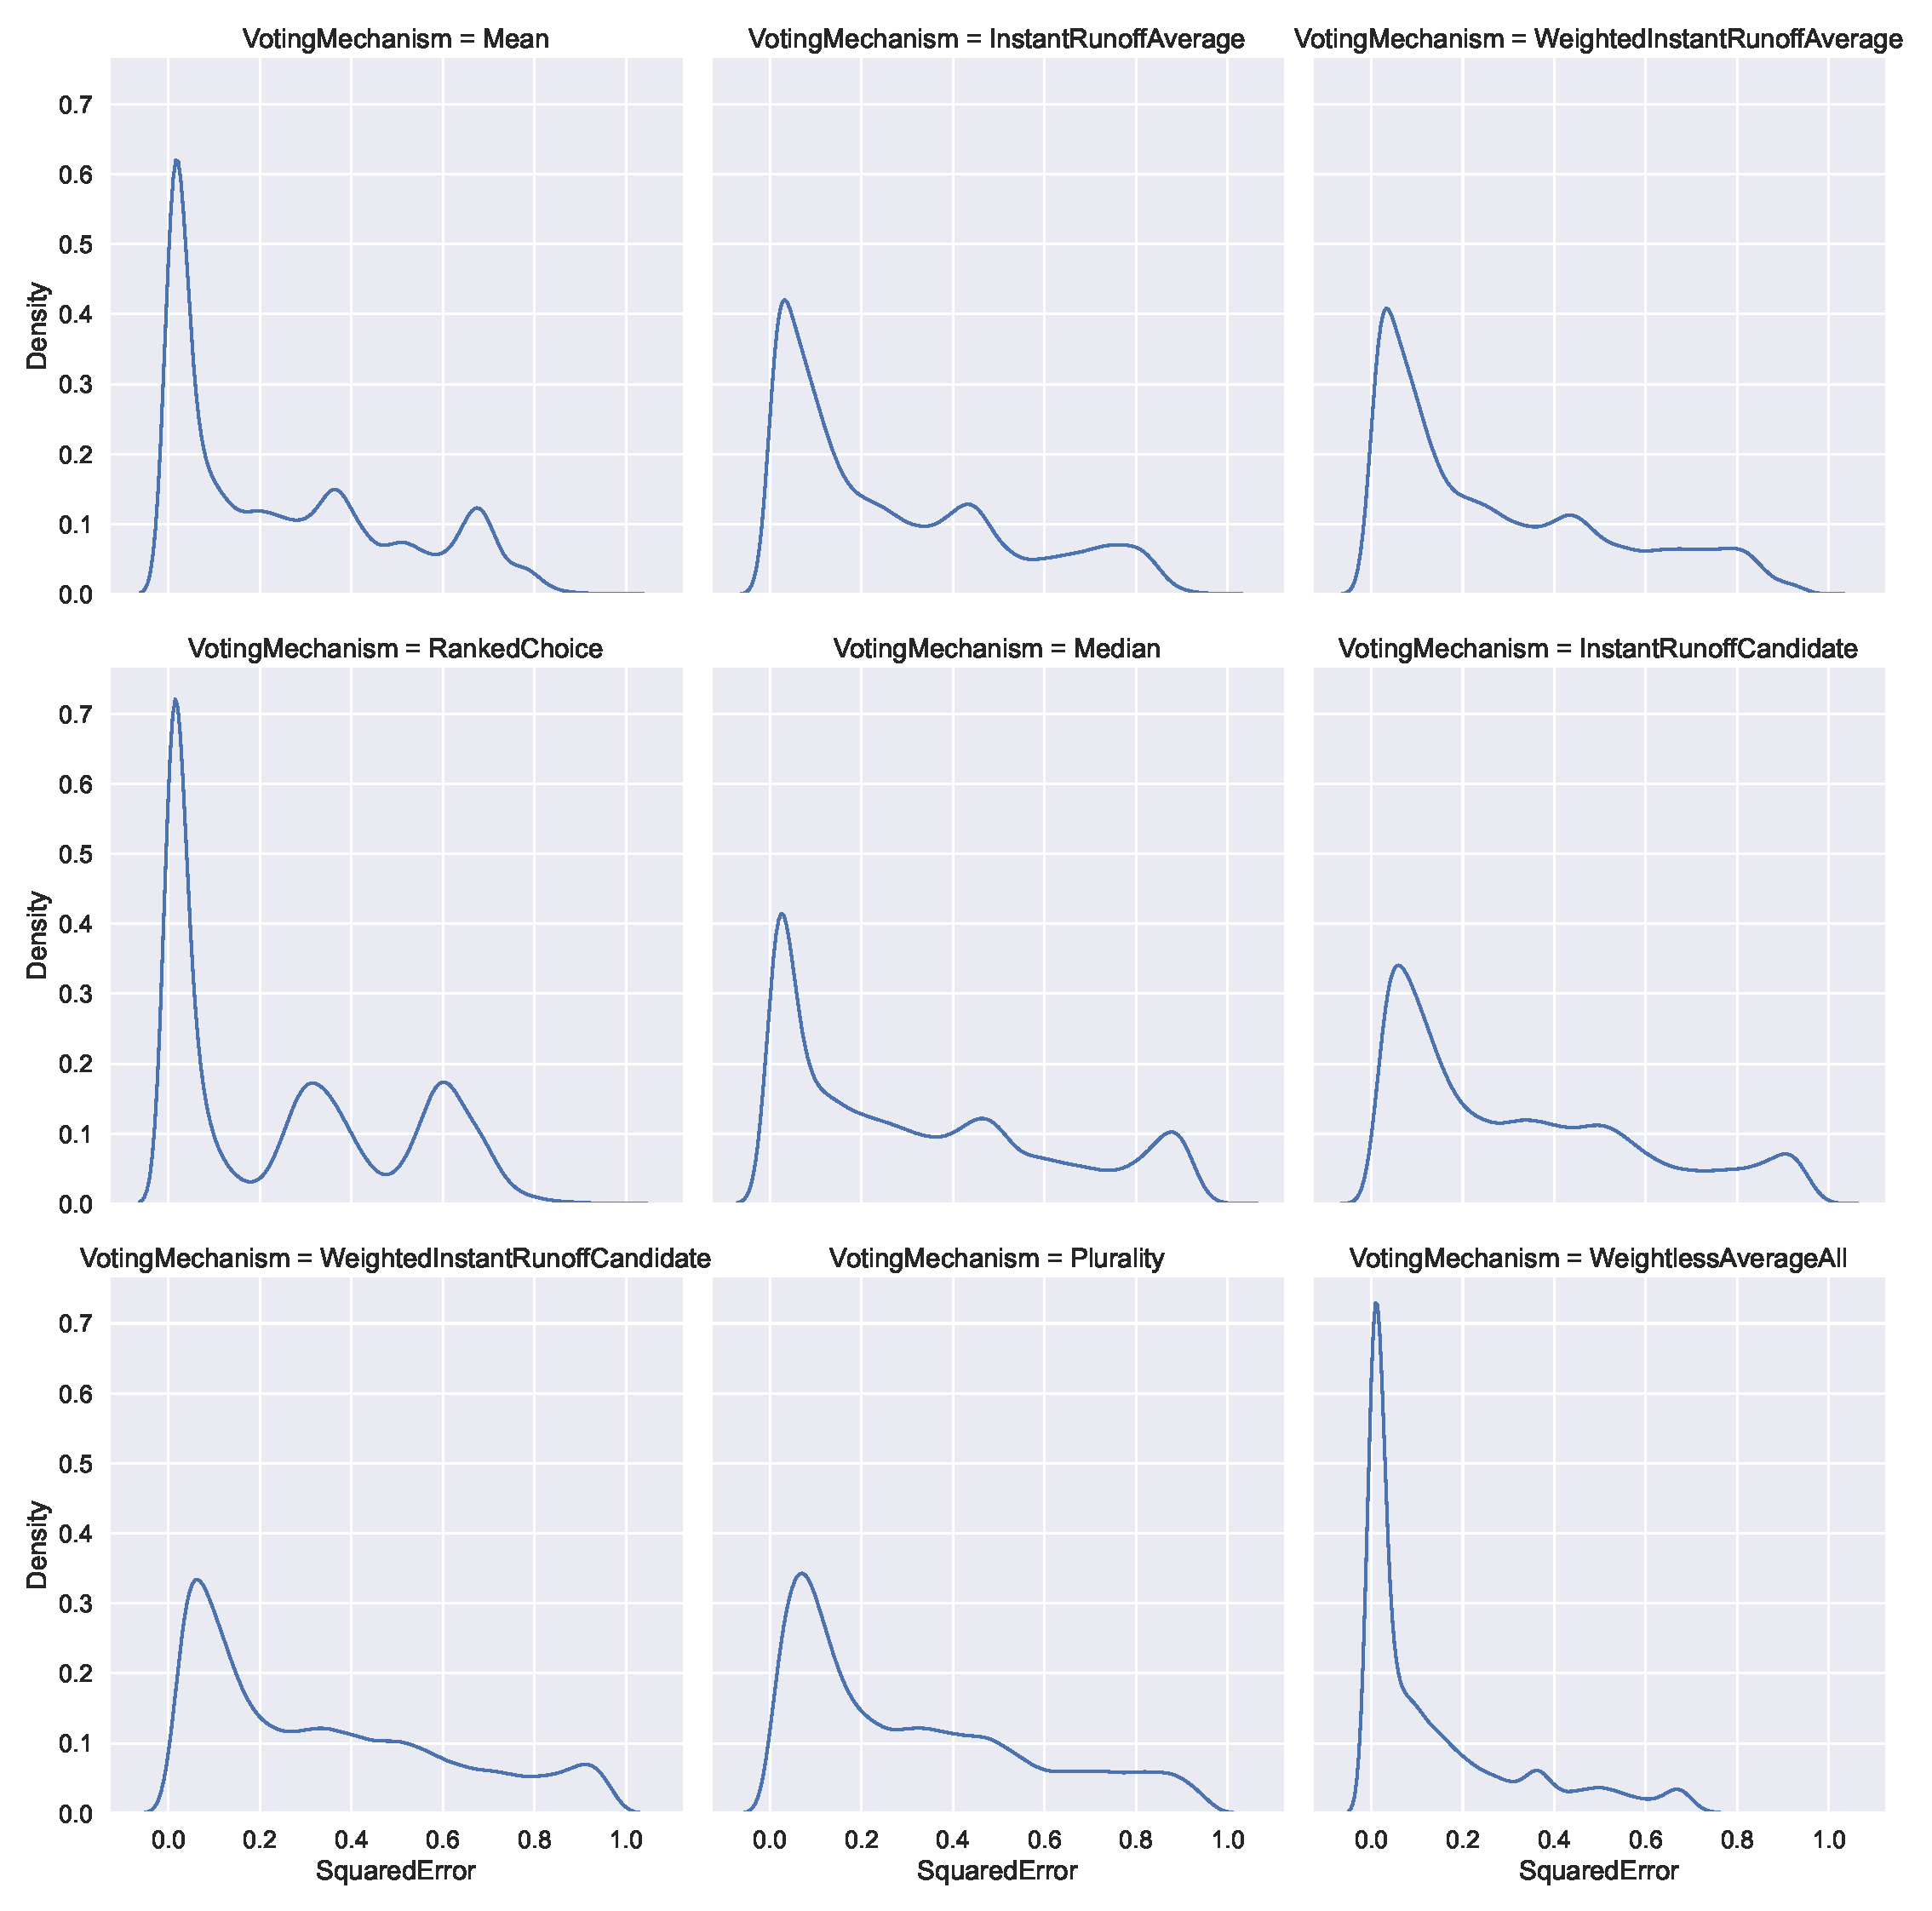
\includegraphics[
        width=\textwidth,
        height=\dimexpr
        \textheight - 2 % Could also be .9\textheight
        \baselineskip,
        keepaspectratio]
    {./content/figures/voting_mechanisms/voting_mechanisms_error_distribution}
    \caption{The distribution of squared error by voting mechanism.}
    \label{fig:voting_mechanisms_error_distribution}
\end{figure}

\begin{figure}[!t]
    \centering
    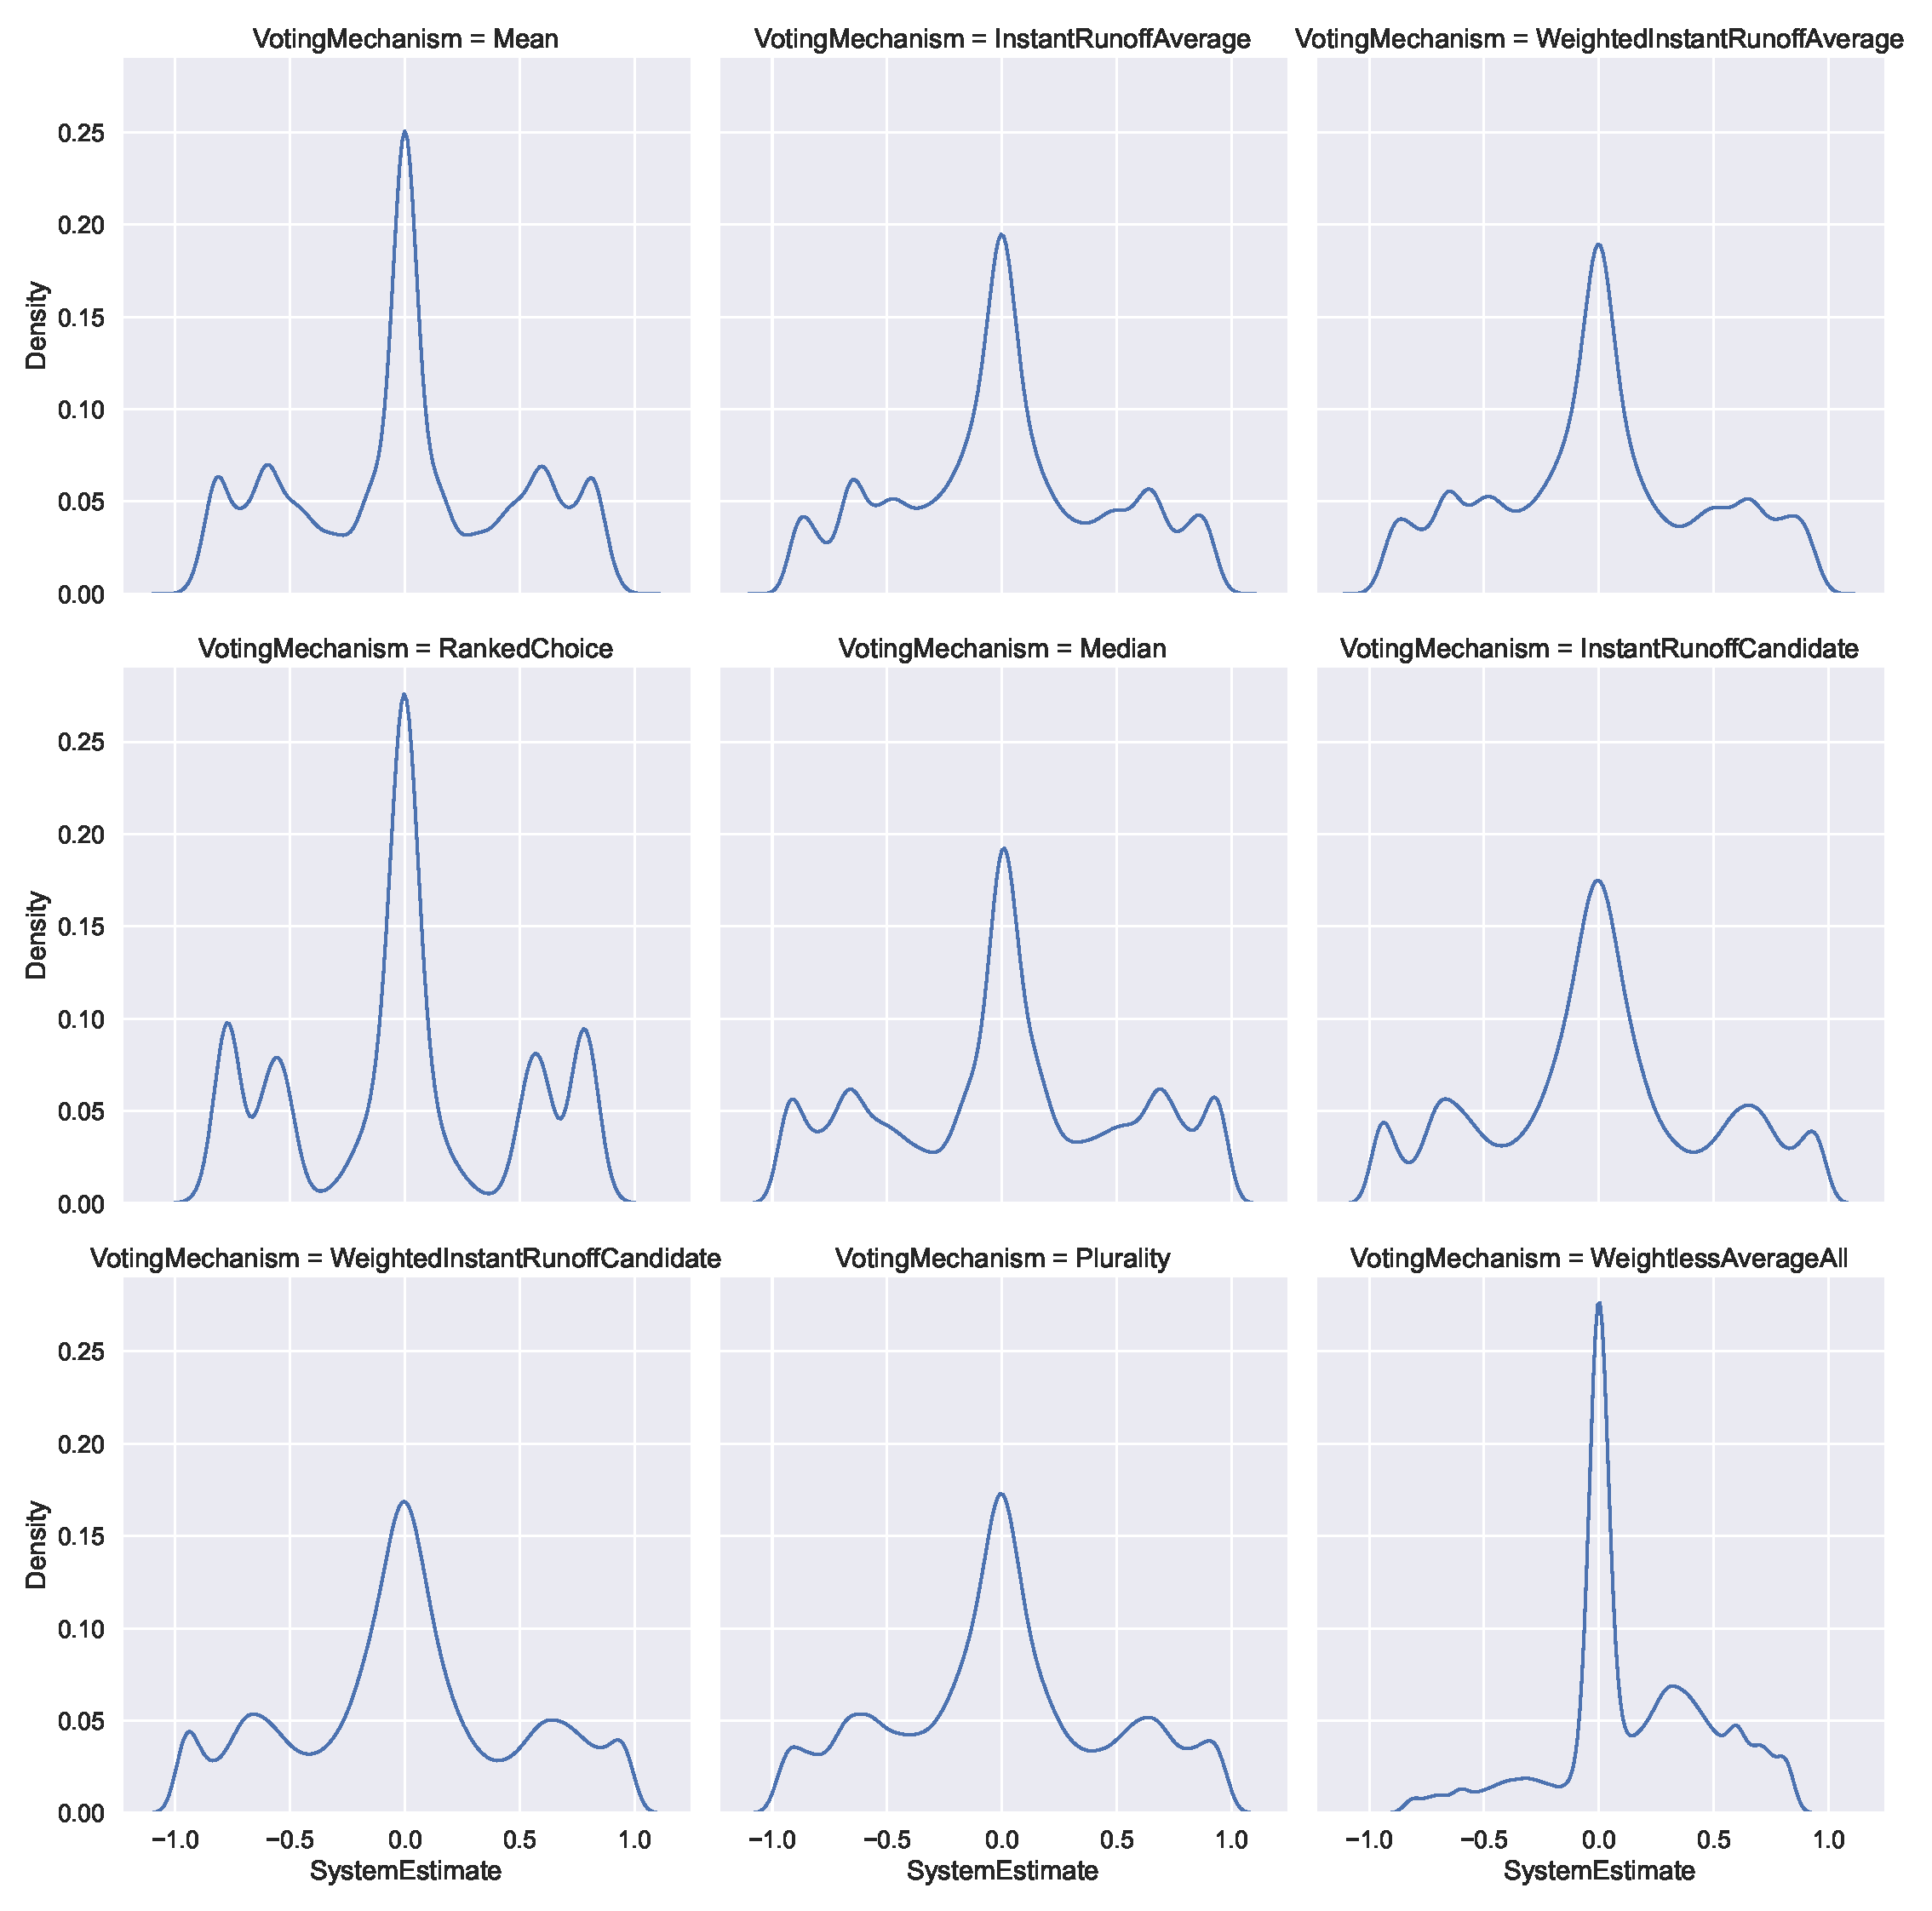
\includegraphics[
        width=\textwidth,
        height=\dimexpr
        \textheight - 2 % Could also be .9\textheight
        \baselineskip,
        keepaspectratio]
    {./content/figures/voting_mechanisms/voting_mechanisms_estimate_distribution}
    \caption{The distribution of system estimate by voting mechanism.}
    \label{fig:voting_mechanisms_estimate_distribution}
\end{figure}

\appendix{Visualizations}\label{chap:visualizations}
\begin{figure}[htbp]
    \centering
    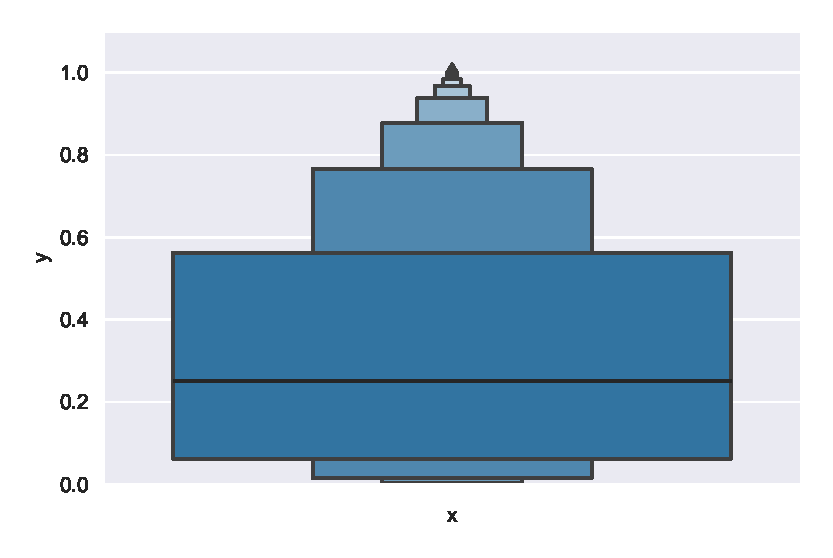
\includegraphics[scale=0.5]
    {./content/figures/expected_even_distribution_squared_error}
    \caption{Expected squared error distribution given a uniform distribution
    of estimates.}
    \label{fig:expected_even_distribution_squared_error}
\end{figure}

\begin{figure}[htbp]
    \centering
    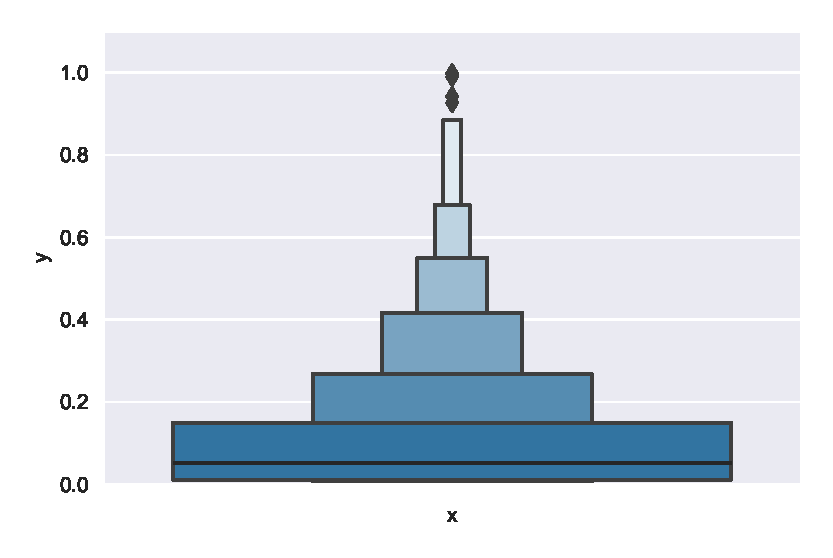
\includegraphics[scale=0.5]
    {./content/figures/expected_gaussian_distribution_squared_error}
    \caption{Expected squared error distribution given a gaussian distribution
    of estimates.}
    \label{fig:expected_gaussian_distribution_squared_error}
\end{figure}

    

%    %
% This is an example of a vita page.  
% Format is not tightly specified. This example comes from Lili Ma.
%
%  Time-stamp: "[vita.tex] last modified by Scott Budge (scott) on 2012-07-16 (Monday, 16 July 2012) at 11:18:06 on goga"
%
%  Info: $Id$   USU
%  Revision: $Rev$
% $LastChangedDate$
% $LastChangedBy$
%

\begin{vita}

\begin{center}
{\Large \bf Michael D. Hegerhorst}\\
\end{center}

\section*{Published Journal Articles}
    \begin{itemize}
    \item Rational Radial Distortion Models of Camera Lenses with Analytical Solution for Distortion Correction, Lili
    Ma, YangQuan Chen, and Kevin L. Moore, {\it International Journal of Information Acquisition}, {\it Accepted}.

    \item A Small Mobile Robot for Security and Inspection Operations, N.S. Flann, K. L. Moore, and Lili Ma, {\it Control Engineering Practice}, vol. 10, pp. 1265-1270,
    2002.
    \end{itemize}

\section*{Published Conference Papers}
    \begin{itemize}
    \item Range Identification for Perspective Dynamic Systems Using
      Linear Approximation, Lili Ma, YangQuan Chen, and Kevin
      L. Moore, in {\it Proc. IEEE Int. Conf. on Robotics and
        Automation (ICRA)},
    2004.
  \item Range Identification for Perspective Dynamic System with
    Single Homogeneous Observation, Lili Ma, YangQuan Chen, and Kevin
    L. Moore, in {\it Proc. IEEE Int. Conf. on Robotics and Automation (ICRA)},
    2004.
  \item Blind Detection and Compensation of Camera Lens Geometrical
    Distortions, Lili Ma and YangQuan Chen, {\it SIAM Imaging
      Science}, 2004.
  \item Flexible Camera Calibration Using a New Analytical Radial
    Undistortion Formula with Application to Mobile Robot
    Localization, Lili Ma, YangQuan Chen, and Kevin L. Moore, in {\it
      Proc. Int. Symposium on Intelligent Control (ISIC)}, 2003.
  \item Sonar and Laser Based HIMM Map Building for Collision
    Avoidance for Mobile Robots, Lili Ma and Kevin L. Moore, in {\it
      Proc. International Symposium on Intelligent Control (ISIC)},
    2003.
  \item Wireless Visual Servoing for ODIS - An Under Car Inspection
    Mobile Robot, Lili Ma, Matthew Berkemeier, YangQuan Chen, Morgan
    Davidson, Vikas Bahl, and Kevin L. Moore, in {\it Proc. IFAC World
      Congress}, Spain, July, 2002.
  \item Visual Servoing of an Omni-Directional Mobile Robot for
    Alignment with Parking Lot Lines, Matthew Berkemeier, Morgan
    Davidson, Vikas Bahl, YangQuan Chen, and Lili Ma, in {\it Proc.
      IEEE Int.  Conf. on Robotics and Automation (ICRA)}, May 2002.
  \item Some Sensing and Perception Techniques for an Omnidirectional
    Ground Vehicle with a Laser Scanner, Zhen Song, YangQuan Chen,
    Lili Ma, and You Chung Chung, in {\it Proc. IEEE Int. Symposium on
      Intelligent Control (ISIC)}, October 2002.
  \item A Small Mobile Robot For Security and Inspection Operations,
    Flann NS, Moore KL, and Ma L, in {\it Proc. IFAC Conference on Telematics
      Applications in Automation and Robotics}, July 2001.
    \end{itemize}

\end{vita}
  % FIXME: I don't think I actually need this unless I'm a doctorate.
    %}}}
\end{document}
